\documentclass[a4paper,12pt]{report}


% Maths packages
\usepackage{verbatim, amsmath, amsfonts, amssymb, amsthm}

% Allows the use of extra characters
\usepackage{textcomp} 

\usepackage[toc,page]{appendix}

% Formatting for URLs
\usepackage{url} 

\usepackage{natbib}

\usepackage{graphicx}

\usepackage[it]{caption}

% PDF referencing
\usepackage[
	hyperindex=true,
	pdftitle={Map the Debate},
	pdfauthor={Joseph Root},
	colorlinks=false,
	pagebackref=false,
	citecolor=blue,
	plainpages=false,
	pdfpagelabels
]{hyperref} % colourlinks=false for printing

% Acknowledgements section
% \usepackage{additional/acknowledgements}

% Chapter title's font and spacing
% \usepackage[times]{quotchap}
% \renewcommand*\sectfont{\minionfont\scshape}
% \renewcommand{\chapterheadstartvskip}{\vspace*{-2.5\baselineskip}}
% \renewcommand*{\chapterheadendvskip}{\vspace{1.3\baselineskip}}

% Packages for type setting
\usepackage{fontspec}
\usepackage[parfill]{parskip}
\usepackage{titlesec}
\usepackage{titling}
\usepackage{textcase}
\usepackage{color}
\usepackage[british]{babel}
\usepackage{setspace}

% Basic typesetting
\setmainfont[Mapping=text-text, Ligatures={Common}]{Adobe Caslon Pro}
\setromanfont[Mapping=text-text, Ligatures={Common}]{Adobe Caslon Pro}
\setmonofont[Scale=0.87]{Consolas}
\setlength{\parindent}{9pt}

% Initialise font families
\newfontfamily\minionfont[Mapping=text-text, Ligatures={Common}]{Minion Pro}
\newfontfamily\trajanfont[Mapping=text-text, Ligatures={Common}]{Trajan Pro}
\newfontfamily\sabonfont[Mapping=text-text, Ligatures={Common}]{Sabon LT Std}
\newfontfamily\caslonfont[Mapping=text-text, Ligatures={Common}]{Adobe Caslon Pro}
\newfontfamily\minionoldfont[Mapping=text-text, Ligatures={Common}, Numbers=OldStyle]{Minion Pro}
\newfontfamily\dinfont[Mapping=text-text, Ligatures={Common}]{DIN 30640 Std}
\newfontfamily\museofont[Mapping=text-text, Ligatures={Common}, Scale=1.2]{Museo Sans 100}
\newfontfamily\consolasfont[Mapping=text-text, Ligatures={Common}]{Consolas}

% Section title's font and style
\titleformat*{\section}{\Large\minionoldfont\addfontfeature{LetterSpace=2}}
\titleformat*{\subsection}{\large\minionoldfont\addfontfeature{LetterSpace=2}}
\titleformat*{\subsubsection}{\normalsize\itshape\minionoldfont\addfontfeature{Scale=1.05}}

\titlespacing*{\chapter}{0pt}{-30pt}{30pt}
\titleformat{\chapter}[display]
	{\flushright\Huge\color{grey}\sabonfont\addfontfeature{Scale=4.5}\bfseries}
	{\thechapter}
	{10pt}
	{\normalfont\flushright\LARGE\color{black}\minionfont\scshape\MakeUppercase}

\titleformat{\part}[display]
  {\LARGE\color{darkgrey}\minionfont\addfontfeature{LetterSpace=3}\scshape}
  { }
  {0em}
	{\MakeUppercase\partname{} \thepart\MakeUppercase { } \vline { }  \color{black}\MakeUppercase}


\definecolor{lightblue}{RGB}{144,164,174}
\definecolor{darkgreen}{RGB}{72,146,0}
\definecolor{lightred}{RGB}{169,53,53}
\definecolor{grey}{gray}{0.55}
\definecolor{darkgrey}{gray}{0.45}

% Code formatting
\usepackage{listings}
\lstloadlanguages{Ruby}
\lstset{
	basicstyle=\consolasfont\color{black}\footnotesize,
	numbers=left,
	numberstyle=\consolasfont\color{grey}\footnotesize,
	commentstyle=\color{darkgreen},
	keywordstyle=\color{blue},
	stringstyle=\color{lightred},
	frame=lines,
	framesep=3pt,
	abovecaptionskip=4pt,
	belowcaptionskip=4pt,
	breaklines=true,
	captionpos=t
}

\setcounter{secnumdepth}{3}

% Details for cover page
\author{Joseph Root\\
Imperial College, London\\
jsr08@ic.ac.uk}
\date{June 2011}
\title{Map the Debate}

\includeonly{title/title, background/background, introduction/introduction}

\begin{document}
	
	\begin{titlepage}

\begin{center}

\vspace*{\fill}
% Upper part of the page


\minionfont\addfontfeature{Scale=1.1}\Huge Map the Debate \\[0.3cm]

\caslonfont\addfontfeature{Scale=1.1}\normalsize Understanding the web's response \\[1cm]

\caslonfont

\emph{Author:} Joseph Root <jsr08@ic.ac.uk>\\
\emph{Supervisor:} Francesca Toni <f.toni@ic.ac.uk>\\ [1cm]
June 2011 \\[3cm]


% 
% % Title
%  \\[0.4cm]
% { \huge \bfseries Lager brewing techniques}\\[0.4cm]
% 
% \\[1.5cm]
% % Author and supervisor
% \begin{minipage}{0.4\textwidth}
% \begin{flushleft} \large
% \emph{Author:}\\
% John \textsc{Smith}
% \end{flushleft}
% \end{minipage}
% \begin{minipage}{0.4\textwidth}
% \begin{flushright} \large
% \emph{Supervisor:} \\
% Dr.~Mark \textsc{Brown}
% \end{flushright}
% \end{minipage}

\vspace*{\fill}

% Bottom of the page
\scshape Imperial College London

\end{center}

\end{titlepage}

	\chapter*{abstract}
	Lorem ipsum dolor sit amet, consectetur adipisicing elit, sed do eiusmod tempor incididunt ut labore et dolore magna aliqua. Ut enim ad minim veniam, quis nostrud exercitation ullamco laboris nisi ut aliquip ex ea commodo consequat. Duis aute irure dolor in reprehenderit in voluptate velit esse cillum dolore eu fugiat nulla pariatur. Excepteur sint occaecat cupidatat non proident, sunt in culpa qui officia deserunt mollit anim id est laborum.
	
	\chapter*{acknowledgements}
	% Parents, Elizabeth, Tim, Catherine, Susan, Francesca. 
	I would like to thank my parents, girlfriend, Tim (sorry!) and Catherine for all their support over the past few months. I can't tell you how much of a difference each one of you has made. It's meant everything to me and I wish I was penning your names to a better project! I'd like to thank Susan for her continual advice, support and open door over the past three years. I couldn't imagine Imperial without you! Thanks also to my second marker Iian for his advice and input. Lastly I'd like to thank my supervisor Francesca. Your cheerful enthusiasm and encouragement has kept me going on the numerous occasions I've felt like giving up. I couldn't have asked for a better supervisor and its (sp?) genuinely been a pleasure.
	
	\tableofcontents
	
	\part{Analysis}
	
	% This is one of the most important components of the report. It should begin with a clear statement of what the project is about so that the nature and scope of the project can be understood by a lay reader. It should summarise everything you set out to achieve, provide a clear summary of the project's background, relevance and main contributions. It should explain the motivation for the project (i.e., why the problem is important) and identify the issues to be addressed (i.e., why the problem is difficult). The introduction should set the scene for the project and should provide the reader with a summary of the key things to look out for in the remainder of the report. When detailing the contributions it is helpful to provide pointers to the section(s) of the report that provide the relevant technical details. The introduction itself should be largely non-technical. It is sometimes useful to state the main objectives of the project as part of the introduction. However, avoid the temptation to list low-level objectives one after another in the introduction and then later, in the evaluation section (see below), say something like "All the objectives of the project have been met blah blah...". A project that meets all its objectives is, by definition, weak and unambitious. Concentrate instead on the big issues, e.g. the main questions (scientific or otherwise) that the project sets out to answer.

\chapter{Introduction}

% The ability to listen to and understand public opinion serves as the foundation upon which democratic society is built. Although the merits of different electoral systems can be debated, in general they all provide effective and functional methods for democratically electing governments. 

\section{Motivation}

From women's rights to civil rights, the influence of public opinion on government policy has been pivotal. Within a healthy democracy the voice of the electorate should be heard and recognised by those chosen to represent them. Throughout history platforms have often been provided for public opinion to be made known, from the early public forums of Greece and Rome, to speaker's corner and the house of commons today. Providing a means for people to express their opinion enables them to both challenge and shape the direction their elected governments take. Finding ways of gathering and understanding this opinion has increasingly proven fundamental if a government wishes to be successful.

Current methods of measuring opinion are largely statistical, with methods such as polling looking at the opinion of a sample group, before using their results to make further predictions. These can be very accurate, however their small sampling rates mean that figures can often be askew. Furthermore polling is both costly and time consuming to conduct, and thus can neither be used to find opinion on breaking news or on a variety of topics. None the less, as methods for measuring public opinion have increased both in accuracy and detail, politicians and policy makers are starting to look to them not only for affirmation of their policies, but for guidance and new initiative.

As the web has become more prevalent throughout society, it is increasingly becoming a platform for discussion and opinion. The initial growth of blogging demonstrated the web's ability to serve as a forum for debate and opinion. However the technical knowledge required to start a blog, alongside the time required to write a post meant that adoption was limited. In the past two years we have seen the rise of micro-blogging (essentially 140 character blog posts) through services such as Twitter. These have seen unprecedented levels of adoption, with Twitter's 200 million users posting 25 billion micro-blog posts in 2010. Due to the simple nature of writing short posts, micro-blog discussion tends to break quickly around news topics, and offers genuine insight into public opinion surrounding news topics.

This project hopes to utilise the growth of publicly available opinion on the web, using it as a source upon which new methods for analysing and measuring public opinion can be built. In particular the project will focus on understanding sentiment on micro-blogging services such as Twitter.

\section{Contributions}

\begin{enumerate}

\item Ruby implementation of a sentiment analysis engine based upon current research. The engine should be able to correctly identify sentences containing sentiment, and classify the sentiment as positive or negative. Different implementations should be tested and compared to determine which algorithms and techniques work best.

\item An algorithm for classifying sentiment as a range of emotion and feeling, rather than just a score along a scale of positive to negative. The algorithm should be implemented in Ruby and included in the sentiment analysis engine.

\item Research optimisations for current algorithms, in order to tailor the sentiment analysis engine for micro-blog posts from services such as Twitter. These optimisation should be implemented within the engine.

\item Research optimisations for current algorithms, in order to better facilitate the understanding of Politically focussed micro-blog data. These optimisation should be implemented within the engine.

\item A Ruby based Twitter module to store and classify live data from Twitter. 

\item Visualisations should be designed and implemented to help better understand the data and classification results.

\end{enumerate}
	
	% The background section of the report should set the project into context by relating it to existing published work which you read at the start of the project when your approach and methods were being considered. There are usually many ways of solving a given problem, and you shouldn't just pick one at random. Describe and evaluate as many alternative approaches as possible. The published work may be in the form of research papers, articles, text books, technical manuals, or even existing software or hardware of which you have had hands-on experience. Your must acknowledge the sources of your inspiration. You are expected to have seen and thought about other people's ideas; your contribution will be putting them into practice in some other context. However, avoid plagiarism: if you take another person's work as your own and do not cite your sources of information/inspiration you are being dishonest; in other words you are cheating. When referring to other pieces of work, cite the sources where they are referred to or used, rather than just listing them at the end. Make sure you read and digest the Department's plagiarism document .

% In writing the Background chapter you must demonstrate your capability of analysis, synthesis and critical judgement. Analysis is shown by explaining how the proposed solution operates in your own words as well as its benefits and consequences. Synthesis is shown through the organisation of your Related Work section and through identifying and generalising common aspects across different solutions. Critical judgement is shown by discussing the limitations of the solutions proposed both in terms of their disadvantages and limits of applicability.

\chapter{Background}
\label{background}

From its early forums through to the 'social web' of today, the Internet has served as a continually expanding platform for discussion. The result has been an explosion in the amount of readily available, computer-formatted textual opinion. With this growth has come an increasing desire to computationally understand the wealth of opinion now so easily accessible. Combining elements of linguistics, natural language processing and machine learning, this field of exploration has come to be known as \emph{opinion mining} or \emph{sentiment analysis}. In the following chapter we will first briefly examine Twitter as a backdrop to our discussion on sentiment analysis. We will then go on to explore the general problems posed by sentiment analysis along with the common approaches and solutions taken in addressing them. In sections \ref{background:discovering_opinion} - \ref{background:topic_extraction} we will discuss in detail the areas and methods of sentiment analysis which will bear relevance to this project's Twitter-based setting. In section \ref{background:emotion} we will explore emotion in general, particularly looking at its scope and ways of classifying it. Finally in section \ref{background:tools} we shall discuss our project's choice of programming languages and tools.

\section{Twitter}
\label{background:twitter}

Twitter is a social-networking web-service. It enables users to post and read 140 character messages known as \emph{tweets}. A user's \emph{timeline} serves as a publicly viewable history of their tweets. Furthermore if someone chooses to \emph{follow} another user, they will be notified of changes to that user's timeline. This simplicity has seen Twitter's user-base rapidly expand, with over 200 million active users today. From football transfers to uprisings Twitter has become the go-to service for spreading news quickly and efficiently.

Since its launch in 2006, certain protocols have emerged from within the Twitter community. These have been embraced by Twitter, enabling it to serve not only as an efficient platform for spreading news, but also as a rich and sophisticated medium for conversation. Notable protocols include:

\begin{description}
	\item [Hashtags] enable users to tag their tweets with any word or combination of characters they deem appropriate. Although this may seem basic at first, through common hashtags, it enables users to take part in a community-wide discussion. For example, during the recent voting reform referendum, the hashtags '\emph{\#yes2av}' and '\emph{\#no2av}' were used to form a debate on the strengths and weaknesses of the Alternative Vote. 
	\item [Mentions] allow users to reference other users in their tweets. Furthermore if a user is mentioned in a tweet, Twitter will notify the mentioned user. Through this, Twitter users can take part in a direct conversations with one or more other users. For example, if we wanted to ask Stephen Fry a question, we could tweet '\emph{what are you eating for breakfast @stephenfry?}'.
	\item [Re-tweets] give users the ability to re-post other users' tweets in their own timeline. This simple feature has had a significant impact on Twitter's ability to facilitate the rapid spread of news. For example in 2009 when the US Airways flight 1549 crash landed in the Hudson river, rapid re-tweeting of an amateur photo meant the news broke on Twitter far earlier than it did within the media at large. This has continued to be true for many more notable events such as the recent North-African revolutions.
	\item [Links] have always been the popular subject of tweets, however the introduction of link-shorteners has changed the way in which they are posted. In freeing up characters by shortening a URL, users now have the option to describe or comment on the link they are tweeting. This has enabled users to engage in deeper conversation on content they have viewed online, and has neatly allowed Twitter's viral nature to better merge with its community's desire for debate.
\end{description}

Through Twitter's RESTful API \footnote{RESTful APIs allow developers to retrieve, modify, create and delete data by making get, post and delete HTTP requests to specified web addresses.}, this rich resource of live news and debate will serve as the project's main data source.

\section{Sentiment analysis}
\label{background:sentiment_analysis}

Sentiment analysis as a field, is the exploration of how we can computationally understand opinions expressed within a body of text. In order to do this, we must first define a computational structure for expressing opinions. In general \cite{Liu:2010tm} this is done by breaking an opinion down into four parts. Firstly we must determine the opinion's focus of discussion, also known as its \emph{topic}\footnote{This is more commonly referred to within literature as an opinion's \emph{feature}, however to avoid later confusion with the machine learning term, we will use the term \emph{topic}.}. This in practise can encompass anything from Government policy to mobile phone battery life. Often opinion is not necessarily that of the author, but of a referenced person or group, therefore it is important to determine the opinion's \emph{holder}. Along with this it is also often necessary to determine the \emph{time} at which the opinion was expressed. Finally, we hope to \emph{classify} (or in some cases quantify) the opinion which has been passed. Leading research \cite{Pang:2002tu,Turney:2002vv} has typically focussed on discrete classification, such as deciding whether an opinion is positive, negative or neutral. A fifth \emph{object} component is sometimes introduced for larger documents, which serves as an identifier for related topics. For example, within a phone review the majority of opinions may share the same object, in this case the phone, but focus on different topics such as battery life or call quality. 

How do we computationally discover opinions and identify their parts? In general the approach can be loosely split into two components, \emph{sentence-level classification} and \emph{document-level classification}. Sentence-level classification determines whether a sentence expresses an opinion along with classifying that opinion if it exists. Furthermore if an opinion is found, sentence-level classification will try to determine its topic, holder and the time at which the opinion was cast. Document-level classification goes on to collate the sentence-level results, in order to form a general description of the document's sentiment. Both these approaches draw heavily upon machine learning techniques. It is important to note here however, a core criticism of the field. Linguists such as Chomsky \cite{norvig} observe that rather than truly trying to understand how sentiment is expressed within language, the field instead takes a statistical, and in his opinion, uninformed approach. This means that rather than determining sentiment by understanding the constructs which have formed it, the field uses a limited linguistic understanding to predict sentiment based upon past examples. Nonetheless, redefining natural language processing and sentiment analysis is not within the scope of this project, and we shall proceed with the field's successfully tried and tested approaches.

As we shall discuss in more detail in chapter \ref{subjectivity}, only sentence-level classification is relevant to this project. Furthermore, methods for determining an opinion's holder and time are unnecessary and will not be discussed here. The remainder of this section will instead focus on the three relevant topics from within sentence-level classification. Firstly we shall explore what exactly an opinionated sentence is and how we can computationally determine this. Next we will look at common approaches to classifying sentiment, before finally examining how we determine the topic of an opinion. Before this however, we shall briefly outline the concepts and methods of \emph{supervised learning} as this shall form the core for each of our classification problems.

\section{Supervised learning}
\label{background:supervised_learning}

Supervised learning is a task within machine learning which infers a function from a set of training data. This approach is well suited to classification problems, and in our case is particularly relevant in discovering opinion and determining polarity. Thus, the remainder of this section will discuss supervised learning with respect to the classification of sentences. 

\subsection{Defining the problem}

In both discovering opinion and determining polarity we want to find an approximate hypothesis function $h$, for an actual function $c$, where $c$ would perfectly perform either task. Both functions will map an input sentence $s\in S$, to a discrete classification $o\in O$, where $S$ is the set of all possible sentences and $O$ is the set of all possible classifications, for example $O=\{positive, negative\}$, such that:

\begin{equation}
	h \approx c:S \rightarrow O
\end{equation}

In order to find our best fit hypothesis function $h$, we will first need to determine a set of \emph{features} for our sentences. Within machine learning, features are the attributes which best describe and discriminate our input data when trying to classify it. For example if we are trying to learn a function to decide whether we should play tennis or not, features might include humidity and sunlight. In essence we want to identify a list of the most useful features $f_1, f_2,\dots,f_n$ for our sentences, such that:
	
\begin{equation}
	h \approx c : \langle f_1, f_2,\dots,f_n \rangle \rightarrow O
\end{equation}

Once a set of features has been chosen we can approximate $h$ by training it. In order to find the perfect hypothesis function for classifying subjective functions, i.e. $h=c$, we would require knowledge of every single possible sentence along with its correct classification. Clearly we could never produce the set of all possible sentences, let alone determine every sentence's classification. Instead, we select a sample of training sentences $T \subseteq S$, and manually \emph{label} each sentence $t \in T$ with a classification $l \in O$. This is our \emph{training data} $D$, such that:

\begin{equation}
	D = \{(t, l) : \forall t \in T \textit{ there exists a manually labelled classification $l$} \}
\end{equation}

Given this training data we can now determine as accurate a hypothesis function as possible for classifying \emph{all} sentences. There are numerous, largely statistical methods for training our hypothesis function. Each brings their own positives and negatives, and there has been extensive research \cite{Pang:2004us} into which methods perform best for opinion based classification. We will discuss the most appropriate methods, features and training data for each classification problem in their respective parts.

\subsection{Naive Bayes Classifier}

The \emph{Naive Bayes (NB)} classifier is a probabilistic supervised classifier \cite{Rish:2001vu}. Using Bayes' theorem, it statistically predicts an input's most likely classification based upon previous experience. Thus given an input represented as the feature set, $f_1, f_2,\-\dots\-,f_n$, a Naive Bayes classifier will essentially classify it with label $o \in O$, according to:

\begin{equation}
	\argmax_{o \in O} \Pr(o | f_1, f_2,\dots,f_n)
\end{equation}

In order to be able to predict this probability, the classifier learns from its training data, which is also represented as a series of feature sets. 

Within sentiment analysis literature \cite{Pang:2008wj,Liu:2010tm}, Naive Bayes classifiers are often experimented with, and unlike in more genral applications \cite{ChihWeiHsu:2002gr}, it often performs strongly. Naive Bayes classifiers also have the additional advantage of requiring only a limited amount of training data in order to be able to perform well.

\subsection{Support Vector Machines}

Unlike Naiver Bayes classifiers, \emph{Support Vector Machines (SVM)} are non-probabilistic, binary classifiers. Given a set of training data presented as feature sets, $f_1, f_2,\dots,f_n$, SVMs hope to find a hypothesis function which best divides the training data into its two respective classes \cite{Lin:2004th}. In essence, this is done by plotting the features in $n$ dimensions, before trying to find the hyperplane which "best" separates the features into their respective classes. In finding the "best" hyperplane, SVMs look for the hyperplane with the largest $n$-dimensional distance between it and it's nearest training example.

As Support Vector Machines present themselves as binary-classifiers, they need to be adapted in order to be able to classify more than two labels. This is referred to as multi-class classification. As outlined by Hsu et al., there have numerous attempts at implementing multi-class classification using SVMs, with each presenting its own benefits. As Caruana et al. observe, typically SVMs outperform NB classifiers, and within sentiment analysis \cite{Pang:2008wj,Liu:2010tm} in particular, Support Vector Machines often perform strongest.

\subsection{Un-supervised learning}

Un-supervised learning is a fairly general term, often used to describe approaches to learning in which there is no labelled data to draw upon on. Typically this means that data is instead clustered based upon attributes known or unknown, to the programmer. As a result of no core underlying approaches, un-supervised learning is difficult to define. However, within this project it shall refer to approaches which use no training data, and in particular those which apply no supervised techniques.

\section{Discovering opinion}
\label{background:discovering_opinion}

In general opinion manifests itself either \emph{explicitly} through \emph{subjective} sentences and phrases, or \emph{implicitly} through \emph{objective} sentences and phrases. An objective sentence expresses factual information, whilst a subjective sentence expresses a mental or emotional state, such as a sentiment or belief. A subjective sentence such as, "\emph{I love the NHS, it's bloody marvellous}", explicitly states an opinion. Similarly however, a sentence such as "\emph{Lost my job due to recent Coalition cuts}" although objective, could also be considered an implicit opinion. This clearly poses a difficult challenge for classification, and as Mihalcea et al. \cite{Mihalcea:2007uh} note, it is one which "has often proved to be more difficult than subsequent polarity classification". As observed by Liu \cite{Liu:2010tm} however, opinionated sentences tend to be a subset of subjective sentences. Due to this, the approaches for classifying them are alike and the terms are taken as interchangeable. This is referred to as \emph{subjectivity classification}.

Subjectivity classification is typically achieved through a mix of supervised and unsupervised learning. In general, unsupervised learning is used to bootstrap a relatively small but accurate training set. The bootstrapped training set is then utilised to train a classifier. Numerous feature choices have been proposed for training subjectivity classifiers. We shall first examine some of the the more commonly used features, as discussed by Wiebe et al. \cite{Wiebe:1999cj}:

\begin{description}
	
	\item [Adjectives] tend to be strong indicators of subjectivity, often serving as descriptions or qualifications of opinion. For example the adjectives in, "\emph{the coalition cuts are \textbf{harsh} but \textbf{necessary}}", are clear indications of subjectivity. As Wiebe et al. \cite{Wiebe:1999cj} observe, a simple binary feature alone - noting the appearance of one or more adjectives - results in a classification accuracy of 56\%. 
	
	\item [Adverbs] modify verbs, adjectives and phrases, for example "\emph{they \textbf{usually} get things right}". Their presence is often an indicator of subjectivity, and although not as useful as adjective presence, their inclusion as a binary feature further improves classification rates. Wiebe et al. \cite{Wiebe:1999cj} suggest a binary feature noting the presence of any adverb other than \emph{not}.
	
	\item [Pronouns] are substitutions for nouns, for example \emph{it} in place of an object. They are often minor indicators of subjectivity, and have been shown to marginally improve classification accuracy when included as a binary feature.
		
	\item [Adjective orientation and gradabilty] tend to be further indicators of subjectivity. Essentially orientation notes whether an adjective encodes a desirable (e.g \emph{beautiful}) or undesirable (e.g. \emph{ugly}) state. The gradability of an adjective denotes the relative extent to which an adjective varies in strength from the norm. For example \emph{"small"} and \emph{"large"} have high gradability. As shown by Wiebe et al. \cite{Wiebe:2000tk}, the presence of polarised, gradable adjectives is a strong measure of subjectivity and a useful feature.
	
\end{description}

Wiebe et al. \cite{Wiebe:1999cj} observed that using the first three features, coupled with a feature noting cardinal numbers presence, resulted in classification rates of 71.2\%. 

But how can we identify these features within a sentence? Adjectives, adverbs and pronouns are all known as \emph{parts of speech (POS)}. A word's POS can take on one of eight roles within a sentence: \emph{verb}, \emph{noun}, \emph{pronoun}, \emph{adjective}, \emph{adverb}, \emph{preposition}, \emph{conjunction} and \emph{interjection}. A word's part of speech is often determined by its position within the sentence. For example "\emph{love}" can be a noun or a verb, dependant upon the context in which it is used. Below is an example of a sentence whose words have been \emph{tagged} with their POS:

\begin{equation}
	\underbrace{{\rm She}}_{\rm pron.} \overbrace{{\rm likes}}^{\rm verb} \underbrace{{\rm big}}_{\rm adj.} \overbrace{{\rm snakes}}^{\rm noun} \underbrace{{\rm but}}_{\rm conj.} \overbrace{{\rm I}}^{\rm pron.} \underbrace{{\rm hate}}_{\rm verb} \overbrace{{\rm them.}}^{\rm pron.}
\end{equation}

\subsection{Part of speech tagging}
\label{background:pos}

Given a phrase or sentence, \emph{part of speech tagging} computationally determines each word's POS. This can be done in variety of ways. Typically basic implementations use a lexicon of words with their appropriate tags, or a more advanced dictionary such as WordNet\footnote{WordNet is a detailed dictionary with additional levels of detail describing the semantic interlinking between words. It will be used throughout this project and shall be discussed in more detail in section \ref{emotion:wordnet}.}. In general these implementations are naive and often simply return a list of possibilities. More intuitive techniques tend to use machine learning to recognise patterns, or are built with a set of linguistic rules. We will discuss the merits of these techniques and their implementation in more detail in chapter \ref{subjectivity}. With a fully tagged sentence it is now possible to build a feature set based upon the relevant parts of speech.

\subsection{Use of supervised techniques}

As noted in our discussion of features, some adjectives are more useful in classifying subjectivity than others. Determining these adjectives, and in this case their polarity, would prove tedious if carried out by hand. Instead, Wiebe \cite{Wiebe:2000ub} suggests a supervised approach using a small set of a hundred or so seed words, such as \emph{good} and \emph{bad}, and a large corpora of text. The corpora is examined for conjunctions, such as "\emph{handsome} and \emph{smart}", and disambiguations such as "\emph{smart but cruel}". When a seed word is found within either scenario, its fellow word's polarity can be inferred. For conjunctions, if one of the words is known as positive, then the unknown word is likely to be positive also. The converse holds for disambiguations, where the unknown word is inferred to be the opposite of the known word. This technique enables the rapid building of a polarised adjective lexicon. It is particularly useful in domains which assign their own meaning to adjectives, for example \emph{sick} is often a positive adjective within youth culture.

Building a training set significant enough for accurate subjectivity classification can often be time consuming. Liu \cite{Liu:2010tm} and Akkaya et al. \cite{Akkaya:2009ww} describe a supervised method for bootstrapping an initial training set. A high precision, low recall rule based classifier, as originally proposed by Wiebe and Riloff \cite{Wiebe:2003wa}, is used to build a small training set from a large corpora. The classifier does this by identifying strong and weak subjective clues within a sentence. If there are two or more strong subjective clues the sentence is classified as subjective. In order to determine objectivity, the sentences on either side are taken into account. If between them neither contain more than one strong and two weak clues, along with no strong clues in the analysed sentence, the sentence is considered objective. If the conditions for subjectivity and objectivity are not met, the classifier leaves the sentence unclassified. The use of supervised methods such as this and the lexicon builder described above are typical within the field. They provide simple and efficient ways of optimising the overall training process.

\subsection{Present research and issues}

Recent literature has also explored numerous improvements to the classic algorithm as described above. One such improvement of notable effect is \emph{subjectivity word sense disambiguation (SWSD)}, originally presented by Wiebe et al. \cite{Wiebe:2006te}, and further refined by Akkaya et al. \cite{Akkaya:2009ww}. SWSD tries to reduce the misclassification of objective words, and thus possibly the sentence, as subjective. These false hits often occur as a result of assuming that if a word exists within a subjective lexicon, it is being used in subjective sense. For example, \emph{pain} is often used subjectively, however within, \emph{early symptoms include body pain}, \emph{pain} is used in an objective sense. SWSD attempts to eliminate this source of error. A subjective lexicon of words is built, and for each of its words, a classifier is trained. Given a potentially subjective word within a sentence, the classifier will label the word's sense as objective or subjective. The classifier is trained using a corpora of sentences whose subjective words have been labelled as either subjective or objective. The classifier is then used to ensure that all subjective words are used in their subjective sense. Using SWSD within subjectivity classification, Wiebe et al. \cite{Akkaya:2009ww} noted a 24\% reduction in error against a classifier using the regular subjectivity lexicon when looking for subjective words. 

Subjectivity classification is a well researched field, however current methods do pose problems. As is typically the case within supervised learning, the classifier's ability is significantly influenced by how representative its training set is of the input domain. Subjectivity classification, along with many other natural language approaches, is often extremely sensitive to the type of content with which it has been trained. This means that if one wants to build a subjectivity classifier for political speeches, the training corpora should be built from similar content, not for example from movie reviews. No fixed approach has been developed for this, and it is an issue we shall have to contend with during our implementation in chapter \ref{subjectivity}. 

\begin{comment}
	
Subjectivity word-sense disambiguation \cite{Akkaya:2009ww}

- typical approaches rely on lexicon of words
	- these are usually word lists rather than meanings (or senses)
	- can lead to false hits i.e. word assumed to imply s, when really it is o
- thus Subjectivity Word Sense Disambiguation
	- labels clue words as subjective or objective sense
	- more feasible than full word-sense
- use SVM
- use bootstrapping to create a training set

- since sentences often contain multiple subjective expressions, expression level classification is more informative than sentence-level classification

Word sense and subjectivity \cite{Wiebe:2006te}
- propose that there are motivations for separate classifiers, one each
- top of page 6 makes very good point about a word typically being subjective, being objective in a subjective sentence

Learning subjective adjectives from a corpora \cite{Wiebe:2000ub}

Effects of adjective orientation \cite{Wiebe:2000tk}
- use word conjunctions to find positive/negative adjectives
	- e.g. would say corrupt and brutal, not corrup or brutal

\end{comment}


\section{Classifying opinion}
\label{background:sentiment_classification}

An opinionated sentence can express a diverse range of sentiment, and classifying this can prove difficult. Sentiment can be classified in numerous ways, for example "\emph{I liked the tone of his speech, however I am uncertain of the proposals within it}", could be interpreted in any number of ways. At a phrase level, we might consider the first part to express some form of delight, while the latter expresses distrust. Of course, to a certain extent these are subjective, and more detailed emotional labels shall be discussed in section \ref{background:emotion}. A more broad classification might classify the first part as positive and the second part as negative. Developing methods for labelling a sentence's polarity has served as a focus for much of the research into classifying opinion. This field is referred to as \emph{sentiment classification}.

But how do we determine sentiment? At first this may seem simple. For example "\emph{I \textbf{love} the EU}" would typically be classified as positive, whilst "\emph{I \textbf{hate} the EU's decentralisation of power}" would be negative. Clearly \emph{love} and \emph{hate} are strong indicators of polarity. Basic methods for classifying sentiment simply check whether any of the words within the sentence exist within a pre-defined polarity lexicon, and classify accordingly. If we explore increasingly complex phrases however, the problem becomes far less simple than simply identifying polarising words. Understanding the scope of negation can present challenges. For example the negative in "\emph{not nice}", simply negates its neighbour, whilst in "\emph{no one thinks that its good}", the ensuing negation spans the phrase. In certain scenarios negation words can even strengthen polarity, such as "\emph{not only good but amazing}". Issues of word sense, similar to those discussed in section \ref{background:discovering_opinion}, present further problems. For example "the National \emph{Trust} may waste money" conveys an opinion which expresses the polar opposite of trust. The domain of the sentiment being expressed can also effect polarity. "\emph{Go read the book}" may be considered positive within a book review, however for a film it is generally see as negative.

At its heart sentiment classification poses a significant linguistic challenge, and the approaches vary as a result of it. They can be broadly split into two approaches however, supervised and unsupervised. Unsupervised methods propose that sentiment can be understood by analysing its linguistic form. By understanding the rules which allow sentiment to be expressed, we should be able to both identify and understand it within a sentence. Supervised methods suggest that the complexities of language make unsupervised methods too specific and difficult to identify. Instead it hopes to make use of machine learning's supervised techniques in order to better classify sentiment. We will explore and contrasts these two methods. In particular, we will focus upon the unsupervised approach put forward by Turney \cite{Turney:2002vv}, and the supervised approach proposed by Pang et al. \cite{Pang:2002tu}.

\subsection{Unsupervised sentiment classification}

Turney \cite{Turney:2002vv} suggests a two part approach to supervised sentiment classification. As discussed when exploring subjectivity in section \ref{background:discovering_opinion}, adjectives tend to be a significant grammatical structure through which sentiment is expressed. Thus, Turney proposes extracting phrases containing adjectives and whose structure indicates an expression of sentiment. Given a sentence, we tag its parts of speech, before extracting any two-word phrases whose structure can be found within the following linguistic patterns:

\begin{table}[h]
	\caption{Extraction patterns for identifying opinionated two-word phrases}
	\label{background:patterns}
	\centering
	\begin{tabular}
		{ l | l l l }
		Rule & First word & Second word & Third word (\emph{not extracted}) \\ \hline
	  1. & JJ & NN, NNS & anything \\
		2. & RB, RBR, RBS & JJ & not NN, not NNS \\
		3. & JJ & JJ & not NN, not NNS \\
		4. & NN, NNS & JJ & not NN, not NNS \\
		5. & RB, RBR, RBS & VB, VBD, VBN, VBG & anything \\
	\end{tabular}
\end{table}

Once these phrases have been identified, we can then determine their sentiment's polarity. This is done by first selecting two words commonly associated with strong positive and negative sentiment. Turney suggests \emph{excellent} and \emph{poor} as the benchmark words for positive and negative polarity. This is largely due to their prevalent use within reviews as descriptions for high and low ratings. In order to calculate a phrases sentiment, we attempt to measure the association between it and benchmark's words. Co-occurence between two words is calculated using their \emph{Pointwise Mutual Information (PMI)}, defined as:

\begin{equation}
	\operatorname{PMI}(word_1, word_2) = \log_2 \left(\frac{\operatorname{p}(word_1 \textit{ \& } word_2)}{\operatorname{p}(word_1)\operatorname{p}(word_2)}\right)
\end{equation}

Where $\operatorname{p}(word_1,word_2)$ is the probability that $word_1$ and $word_2$ co-occur within a corpora, and $\operatorname{p}(word)$ is the probability that $word$ occurs. Now that we have definition for PMI, we can define the \emph{semantic orientation (SO)} of a $phrase$ as:

\begin{equation}
	\operatorname{SO}(phrase) = \operatorname{PMI}(phrase, "excellent") - \operatorname{PMI}(phrase, "poor")
\end{equation}

The resulting semantic orientation is a measure of a phrase's sentiment. An SO larger than 0 denotes positive polarity, while an SO less than zero indicates negative polarity. Thus, a sentence's overall polarity is simply the average of its phrases' SO. This approach to supervised sentiment classification has proven effective across a variety of review domains. Turney reports an impressive 80\% when classifying bank reviews and an even better 84\% accuracy for automobile reviews. He does note however, that movie reviews present a challenge for his supervised approach, reporting an accuracy of 65.83\% within the movie domain. Nonetheless, across domains Turney reports classification rates of 74.39\%, demonstrating the strong potential which lies within unsupervised methodologies.

\subsection{Supervised sentiment classification}

Shortly after Turney published his paper on supervised approaches \cite{Turney:2002vv}, Pang et al. \cite{Pang:2002tu} put forward a counter paper. This addressed the potential of supervised learning within the same domain of internet reviews as Turney's original paper. At its core, Pang et al. address the issue that often sentiment can be expressed in very subtle ways. For example, "\emph{How could anyone sit through this movie?}" does not express negative opinion in any readily apparent way. Essentially the proposition put forward by Pang et al. is that the nuanced structures through which we express opinion are too vast and varied. They cannot simply be whittled down into a simple set of rules, and rather, we should look to experience to guide our classification.

As with any supervised problem, the learning experience is largely guided by our choice of features. Before we examine these, it is important to introduce the concept of \emph{n-grams} and how they work as features. For example, if we use unigram feature set, there is a feature for every possible word. A feature set this large is unnecessary however, as the only words which will be important in classification are those we encounter in training. Thus we build a feature set from the words we encounter when training. If our training set only contained "\emph{I love the NHS}", we would have the following feature set for classification $\langle f_{I}, f_{love}, f_{the}, f_{NHS} \rangle$. Alternatively if we used bigrams (2 word phrases), we would have a feature set $\langle f_{(I,love)}, f_{(love,the)}, f_{(the,NHS)} \rangle$. But what values do we assign to these features when given a sentence to classify? Pang et al. experiment with two options:

\begin{enumerate}
	\item{\emph{Term presence} denotes whether the n-gram phrase that a feature represents occurs within our sentence. For example, using the unigram and bigram feature sets above, and given a sentence "\emph{I hate the NHS}", we would have the following feature sets:
	\begin{eqnarray} 
		& \langle f_{I}, f_{love}, f_{the}, f_{NHS} \rangle = \langle true, false, true, true \rangle \nonumber \\
		& \langle f_{(I,love)}, f_{(love,the)}, f_{(the,NHS)} \rangle = \langle false, false, true \rangle \nonumber
	\end{eqnarray}
	}
	\item{\emph{Term frequency} denotes how frequently each feature's n-gram phrase occurs within our sentence. For example, using the unigram and bigram feature sets above, and given a sentence "\emph{I hate the NHS, but I love my GP}", we would have the following feature sets:
	\begin{eqnarray} 
		& \langle f_{I}, f_{love}, f_{the}, f_{NHS} \rangle = \langle 2, 1, 1, 1 \rangle \nonumber \\
		& \langle f_{(I,love)}, f_{(love,the)}, f_{(the,NHS)} \rangle = \langle 1, 0, 1 \rangle \nonumber
	\end{eqnarray}
	}
\end{enumerate}

Pang et al. also experiment with appending POS tags to the end of each word, thus distinguishing between their possible uses. In order to handle negation, any words between a negative word such as \emph{not} and the next punctuation mark are tagged with a $NOT$. For example "I do not like the NHS" would result in a feature set $\langle f_{I}, f_{do}, f_{not}, f_{NOT-like}, f_{NOT-the}, f_{NOT-NHS} \rangle$. 

The different feature sets were tested within the movie review domain. The presence feature set for unigrams performs strongest in their experiments with an accuracy of 82.9\%. The combination of unigrams and bigrams sees a marginal drop in accuracy to 82.7\%. Interestingly POS tags also have a slight negative effect on accuracy, seeing it drop to 81.9\% when coupled with a unigram presence feature set. In domains where the expression of sentiment is subtle, supervised approached have a clear benefit over their unsupervised counterparts. However, supervised learning requires one to build a training set, which can often prove time consuming. Furthermore its understanding of sentiment is based upon experience, thus it could never really explain why it reached its decision. Deciding which approach is better is difficult, and we shall explore this is more detail in section \ref{polarity}.

\subsection{Present research and issues}

Recent research has focussed on how combinations of supervised and unsupervised learning can be used to improve classification rates. Essentially these improvements have hoped to introduce greater linguistic detail into the supervised approach described by Pang et al.. In the following section we shall provide a general overview of two improved methodologies put forward by Wilson et al. \cite{Wilson:2005tt} and Benamara et al. \cite{Benamara:2007wz}.  We shall explore these approaches in greater detail in section \ref{polarity}.

Although Wilson et al. \cite{Wilson:2005tt} acknowledge the need for elements of supervised learning, they observe that the sentence-level approach put forward by Pang et al. is to general. Instead they propose that to truly understand sentiment, we must approach it at a phrase level. The main motivation behind this is the common misclassification of \emph{clue} words as polar, when the sense in which they are being used means they are in fact neutral. This problem is of particular relevance to the supervised approach discussed above. The method put forward by Pang et al. essentially creates a lexicon of polar words during training and later uses them as clue's for classifying polarity. As mentioned in our introduction to opinion classification, this can lead to words being taken out of context to classify neutral statements as polar. Wilson et al. propose a two step solution to this. The first step identifies all clue phrases within a sentence, before using a supervised approach to classify each one as polar or neutral. The polarity of each polar phrase is then disambiguated to give it an overall classification of either \emph{positive}, \emph{negative} or \emph{both}. Not only does this approach provide a more rigorous framework for sentiment classification, unlike the methods put forward above it also acknowledges the potential neutrality of phrases within a sentence.

Alongside the influential research into phrase-level sentiment by Wilson et al., other prominent research has focussed on measuring sentiment strength. Benamara et al. \cite{Benamara:2007wz} highlight the important role of adverbs as measures of opinion. These adverbs are known as \emph{adverbs of degree}. Within this subset of adverbs, five clear classifications can be noted:

\begin{enumerate}
	\item \emph{Affirmation} adverbs such as \emph{certainly} and \emph{absolutely} strengthen adjectives.
	\item \emph{Doubt} adverbs such as \emph{possibly} and \emph{seemingly} weaken adjectives.
	\item \emph{Strong intensifying} adverbs such as \emph{exceedingly} and \emph{extremely} strengthen adjectives.
	\item \emph{Weak intensifying} adverbs such as \emph{barely} and \emph{scarcely} weaken adjectives.
	\item \emph{Negation/minimising} adverbs such as \emph{hardly} and \emph{rarely} invert or neutralise adjectives.
\end{enumerate}

Using a lexicon containing adverbs of degree and their appropriate classification, all unary and binary adverb adjective combinations are found. A unary combination has the form $\langle adverb \rangle\langle adjective \rangle$, whilst a binary combination has the form $\langle adverb_i, adverb_j \rangle\langle adjective \rangle$. Each adjective in the matching phrases has its polarity strength adjusted according to the classification of the adverbs which proceed it. For unary combinations the score is a product of the adjective and adverb strengths. For binary combinations, the strength of $\langle adverb_j \rangle\langle adjective \rangle$ is calculated first as if it were a unary combination, before calculating the strength combination of the resulting score and $adverb_i$. Benamara et al. report results almost on par with human strength classification, highlighting the proposed method as not only viable but effective.

Although significant improvements have been made within the field, sentiment classification is still far from perfect. Many of its problems have been reduced in size, however they have not been eradicated. One could argue that this is largely due to the statistical nature of supervised learning, and clearly the field still has a lot to learn from linguistics. Most importantly to this project however, is the fact that little research has explored beyond the confines of polarity and into the realm of emotion. We shall explore the field's limited approach to the classification of emotion in more detail later, in section \ref{background:emotion}.

\begin{comment}

Using adverbs for grading - Benamara et al. \cite{Benamara:2007wz} 

Subjectivity does not necessarily imply a polarised opinion

Broad overview in \cite{Pang:2008wj}

Phrase level sentiment analysis \cite{Wilson:2005tt}

Movie reviews, thumbs up/down \cite{Turney:2002vv} \cite{Pang:2002tu}

\end{comment}

\section{Topic extraction}
\label{background:topic_extraction}

Unlike subjectviity and polarity, research into topic extraction is not as well developed or scoped. As a result, the methods for topic extraction tend to be less unified in approach.

Somasunndaran et al. \cite{Somasundaran:2008tw} propose that a sentences topics can be discovered through role labelling. Essentially this takes words such as "\emph{fear}", and assigns the words around it an argument role, based upon a known set of rules. For example fear has two arguments, so in "\emph{we fear death}", argument one is said to be "\emph{we}" whilst argument two is "\emph{death}". Rules such as these are built for a core set of words, so that in any instance the arguments which these roles take can be identified to serve as topics.

Other research such as that proposed by Nigam et al. \cite{Nigam:2004ur} suggests taking a purely supervised approach, in which unigrams are used to indicate whether a word is subjective based upon a prior labelled set. This however is dependant upon a large corpora of labelled data, and furthermore does not make any attempt to understand the linguistic patterns behind how a topic can be identified.

Clearly research is varied, and no concrete work can be offered as an example of a "typical" approach. In many ways this is largely due to the fact that what constitutes a topic is largely dependant upon who is looking for it and why. For example, for politicians looking to understand responses to policy change, the topics they want to identify may be emotional responses whilst for a company examining reviews it might be aspects of their product.

\section{Sentiment on Twitter}
\label{background:sentiment_on_twitter}

With the recent and rapid growth of Twitter has come an interest in understanding the sentiment expressed on it. Although at its heart an issue of sentiment analysis, Twitter's constraints and protocols pose new and different issues for current approaches. Literature is still limited, and solutions to the problems within it are varied. In this section we will focus on some of the more prominent approaches. In particular we will outline the framework proposed by Barbosa and Feng \cite{Barbosa:ws}, whilst looking at some of the innovative improvements and observations put forward by Go et al. \cite{Go:2009ut} and Bermingham et al. \cite{Bermingham:2010vh}.

Barbosa and Feng \cite{Barbosa:ws} propose a two stage sentiment analysis framework. Firstly the subjectivity of a tweet is determined, and if subjective, the tweet's sentiment is then classified. This framework bears many similarities to sentence-level sentiment classification, however the approach within each stage is in many ways very different. Particular emphasis is placed upon the need for strong subjectivity detection. There is a lot of \emph{noise} on Twitter through adverts and spam accounts, thus it is important to filter this out if we ever hope to obtain an accurate overview. A typical noisy tweet might be:

\begin{quote}
	\emph{Get a FREE \$500 Starbucks Gift Card >> Special Online Offer ...: Starbucks is celebrating its first forty years ... http://bit.ly/iepyV5}
\end{quote}

Barbosa and Fang propose some previously unconsidered features for helping distinguish noise from subjective tweets. As evident from analysing the tweet above, Barbosa and Fang note that \emph{link presence} and \emph{uppercase letter frequency} serve as particularly useful subjectivity clues. A novel approach is taken to training the subjectivity classifier using existing online Twitter sentiment classifiers. Subjective tweets are scraped from three such sites, and any tweet appearing as subjective in all three is added to the training data. They report that although this can lead to slight bias, it serves as an effective bootstrapping method. 

Barbosa and Fang take an entirely supervised approach to polarity classification using many of the features discussed in section \ref{background:sentiment_classification}. Uppercase letter frequency again proves particularly useful, along with a feature for \emph{good emoticons}. An emoticon is a text-character face expressing an emotion, for example happy is commonly represented as \texttt{:)} while sad is \texttt{:(}. Barbosa and Fang note significant improvements both in subjectivity and sentiment classification when using tweet-based features, as opposed to the typical approaches described in sections \ref{background:discovering_opinion} and \ref{background:sentiment_classification}. Using unigrams alone for sentiment classification, Barbosa and Fang report an error rate of 44.5\%, whilst the introduction of Twitter based features reduces this to 25.1\%. Although far from perfect, the improvements are notable, and suggest that a better understanding of the intricacies of Twitter could lead to further improvements.

Interestingly, recent work by Bermingham and Smeaton \cite{Bermingham:2010vh} suggests that further linguistic detail when building a feature set in fact harms classification rates. Rather than using POS tagging or larger n-grams, they note that features such as link presence and punctuation mark frequency serve as far better discriminators for subjectivity and polarity. They report accuracy rates of 74.85\%, which are strikingly similar to those achieved by Barbosa and Fang. 

Building a training set for Twitter can prove difficult due to the need for large data sets. There is an extraordinary diversity of structure, language and grammatical approach on Twitter, thus a large training set is necessary if we hope to be able to accurately classify its broad range of opinion. Further to the innovative approach taken by Barbosa and Fang, Go et al. \cite{Go:2009ut} suggest a further innovative technique for quickly building a large data set. By searching Twitter for all tweets containing positive and negative emoticons, Go et al. were able to quickly assemble a list of polarised opinion. This method for building a training set proved remarkably successful, and simply using unigrams as features, they report an accuracy rate of 82.2\%. 

Although literature regarding sentiment analysis on Twitter is limited, there have been significant advances in accuracy. Interestingly, as Bermingham and Smeaton observe, detailed linguistic features seem to be of little benefit when classifying subjectivity and polarity. However, as noted by Go et al., the size of the training set seems to have a marked effect on classification accuracy. Clearly Twitter poses many new challenges for sentiment analysis, and although progress has been made more in depth research is needed before the best approaches can be truly identified.

\begin{comment}

Understanding sentiment on Twitter however, requires slight changes to our approach. We will assume that opinion expressed within a tweet is the user's own, and that the time at which a tweet is posted reflects the time at which any opinion in it was cast. This leaves us with three core problems. First we must determine whether a tweet contains an opinion, and if so, we must be able to both classify it and determine its topic. Research into Twitter-targeted sentiment analysis is limited, however, due to the length constraints placed upon tweets, aspects of sentence-level classification still bare relevance. Furthemore work such as Bermingham' \cite{Bermingham:2010vh} and Barbosa's \cite{Barbosa:ws} highlight some key variations in approach to sentiment analysis on Twitter.

\cite{Barbosa:ws} - suggests 2-step framework, subjectivity detetction then classification
\cite{Barbosa:ws} - additional features from tweet syntax

Robust sentiment detection \cite{Barbosa:ws}
	- good overview

Identifying themes/sentiment \cite{KumarPal:2010fd}
- good topic extraction

Is brevity an advantage? \cite{Bermingham:2010vh}

Sentiment in twitter events \cite{Thelwall:to}

Distant supervision \cite{Go:2009ut}

\end{comment}

\section{Emotion}
\label{background:emotion}

Defining emotion has been a problem that has puzzled philosophers and thinkers as far back as Cicero and Descartes. Although there is no unifying theory, or completely accepted classification, in general many have agreed there to be two broad types of emotion, the \emph{basic emotions} and \emph{complex emotions}. Basic emotions are biologically innate within all humans, whilst complex emotions are culturally specific amalgamations of our basic one. Deciding upon what constitutes both basic and complex emotions however has been the cause of significant debate. Perhaps the two most prominent classifications of recent times are those put forward by Ekman \cite{Ekman:1969ux} and Plutchik \cite{Plutchik:2001tp}. 

\subsection{Current defenitions}

After years of work within the field, and having observed the Fore tribesmen of Papua New Guinea, Ekman's 1969 paper presented what he believed to be the six core emotions. These were \emph{anger}, \emph{disgust}, \emph{fear}, \emph{happiness}, \emph{sadness}, \emph{suprise}. Within his work he notes that the Fore tribesmen could identify these emotions when presented with photos of faces expressing them, regardless of their cultural origin. 

In 1980, Robert Plutchik \cite{Plutchik:2001tp} presented his research into human emotion. Within it, he uses five of the emotions put forward by Ekman, whilst introducing three new emotions (see figure \ref{fig:eight_basic_emotions}). Plutchik expands these emotions further, referring to them as \emph{dimensions}, within which different emotions can express varying degrees of their dimension. Furthermore, each of the eight emotion definitions also has a polar opposite definition within the list.

\begin{figure}
	\caption{Robert Plutchik's eight basic emotions \emph{(* proposed by Ekman)}}
	\label{fig:eight_basic_emotions}
	\centering
	\begin{tabular}{ | l | l | l | l | l |}
		\hline
		Basic Emotion & Polar Emotion & \multicolumn{3}{|c|}{Degrees (strong to weak)}\\
		\hline
		Joy	& Sadness & Ecstasy & Joy & Serenity \\
		Trust	& Disgust & Admiration & Trust & Acceptance\\
		Fear* & Anger & Terror & Fear & Apprehension\\
		Surprise & Anticipation & Amazement & Surprise & Distraction\\
		Sadness* & Joy & Grief & Sadness & Pensiveness \\
		Disgust* & Trust & Loathing & Disgust & Boredom\\
		Anger* & Fear & Rage & Anger & Annoyance\\
		Anticipation* & Surprise & Vigilance & Anticipation & Interest\\
		\hline
	\end{tabular}
\end{figure}

Taking this original list of eight, Plutchik also proposesa further eight complex emotions, formed from combinations of the original eight (see figure \ref{fig:eight-complex-emotions}).

\begin{figure}
	\caption{Robert Plutchik's eight complex emotions}
	\label{fig:eight-complex-emotions}
	\centering
	\begin{tabular}{ | l | l | l | }
		\hline
		Combined basic emotions & Complex Emotion & Polar Emotion \\
		\hline 
		Anticipation \emph{and} Joy & Optimism & Disappointment \\
		Joy \emph{and} Trust & Love & Remorse \\
		Trust \emph{and} Fear & Submission & Contempt \\
		Fear \emph{and} Surprise & Awe & Aggressiveness \\
		Surprise \emph{and} Sadness & Disappointment & Optimism \\
		Sadness \emph{and} Disgust & Remorse & Love \\
		Disgust \emph{and} Anger & Contempt & Submission \\
		Anger \emph{and} Anticipation & Aggressiveness & Awe \\
		\hline
	\end{tabular}
\end{figure}

The level of detail within Plutchik's research provides a wider scope of definition than that put forward by Ekman. For this reason it shall serve as the classification system we attempt to computationally replicate. Furthermore, Plutchik's proposal introduces concepts of polarity and strength to emotion. Both these concepts bare strong similarities to research within sentiment classification \ref{background:sentiment_classification}, and we will explore the benefits of this similarity in chapter \ref{polarity}.

\subsection{Computational classification}

As with defining emotion, approaches to classifying it are broad and in general, differ widely. Each present their own definitions of emotion, and as a result approaches can vary quite widely. Although essentially a machine learning problem, unlike polarity classification for example, emotion classification can not be attributed to one single field. It is commonly researched within Natural Language Processing, however other fields such as Human-computer interaction, also present their own approaches. 

As with most machine learning problems, classifying emotion can be approached both through supervised and un-supervised techniques. Yang et al. \cite{Yang:2007wx} propose a largely unsupervised approach to classification, largely based upon an emotion corpora built with distant supervision. In a similar fashion to Go et al. \cite{Go:2009ut}, blog posts are scraped for sentences containing emoticons. These sentences are then classified with an emotion based upon that which Yang et al. perceive the emoticon to hold. Once done, each word in any sentence containing an emotion is given a point-wise mutual information score, based upon how often it co-occurs with its sentence's emotion. With a corpora of words and their relation to any given emotion now built, Yang et al. classify new sentences by examining their corpora to see if any of the sentence's words exist within it. If any words do exist within their corpora, the sentence's score for the word's emotion is increased. Yang et. al see considerable success with this method, however the diversity of the emotion they can label is limited to measures of \emph{valence} and \emph{energy}. Furthermore, the approach uses no manual annotation when testing, instead relying on its unsupervised labels, and thus it could be seen as merely favouring its own error.

In an alternative approach, Alm et al. \cite{Alm:2005vc} put forward a supervised method for classifying emotion. In training their classifier, Alm et al. manually annotate a corpus of 185 children's stories with one of six emotions, \emph{angry}, \emph{disgusted}, \emph{fearful}, \emph{happy}, \emph{sad} and \emph{surprised}. Interestingly, they note that their annotators only achieved an agreement rate of between 45 and 65\%, suggesting that classification rates such as those seen in subjectivity and sentiment analysis can never truly be achieved. With their corpora now annotated, they draw upon thirty core features for training and classifying. Many of these features are similar to those used in polarity classification such as unigrams and adjectives. However, of particular interest and novelty is their use of WordNet as a feature for exploring how the semantic grouping of a word will effect a sentence's emotional classification. This is done by grouping WordNet words based upon their relation to each of the six emotions. Although Alm et al. do not report the success rates seen in work by Yang et al., their classifier performs well, on average achieving accuracy rates of 63\% when determining whether emotion exists. They are less successful in classifying the actual emotion and are only able to achieve an F-score of 32\% when classifying negative emotions such as fear, and 13\% for positive emotions such as happiness. 

It is clear from the work of Alm et al. \cite{Alm:2005vc} that classifying emotion with any degree of detail or certainty is a remarkably difficult process, and one in which there is a lot of progress still to be made. Although emotion classification across a limited range has seen some success, such as that seen by Yang et al., as one's definition of emotion increases in scope, our ability to accurately classify it drastically falls.

\section{Tools and languages}
\label{background:tools}

Although speed is not the primary performance measure within this project, we still hope to maximise efficiency where possible. This desire to strike a balance between programming practicality and speed has defined our choice of tools and languages. As a result languages have primarily been chosen based upon their practicality with regards to rapid development and experimentation. On the other hand, data critical tools such as database software have been chosen with the hope of maximising efficiency whilst remaining flexible. The remainder of this section will focus upon which languages and tools we have chosen and why, along with any potential pitfalls we may encounter in using them.

\subsection{MongoDB}

MongoDB (www.mongodb.org) is a no-SQL document-oriented database. Essentially, MongoDB discards schemas and relationships, instead leaving us with the complete freedom to structure and organise documents as we choose. Documents (or objects) are stored using \emph{JSON}\footnote{\emph{JavaScript Object Notation is an open standard for defining data structures and objects. Although based upon JavaScript, methods for converting to and from JSON are supported in most languages.}} notation, and can be organised into \emph{collections} of documents. For examples a collection statuses, might consist of a set tweets each stored within MongoDB as JSON objects, such as that in listing \ref{overview:example_json_tweet}.

\begin{lstlisting}[language=Ruby, caption={Example tweet stored within MongoDB}, label=overview:example_json_tweet]
{
	"_id" : ObjectId("4dee4f6697dee90936000082"),
	"text" : "@CalebHowe It wasn't Weiner! http://flic.kr/p/9Rgb84 #weinergate",
	"source" : "twitter_search",
	"source_id" : NumberLong("78133750344597504"),
	"created_at" : "Tue Jun 07 2011 17:18:46 GMT+0100 (BST)",
	"from_user" : "speciallist",
	"from_user_id" : 15966313,
	"to_user" : "CalebHowe",
	"to_user_id" : 8574053
}
\end{lstlisting}

As MongoDB is schema-less, the database makes no structural checks on existing data nor does it check when inserting new data. This means that if there are discrepancies such as additional fields, the database will neither complain or alert the user. 

The simplicity of document-oriented databases has led to a rapid adoption amongst data-driven companies\cite{popescu, moore}, preferring versatility and speed over the benefits of relational databases. With this has come increasing research and stability, ensuring that databases such as MongoDB are not only fast and efficient, but stable and safe. MongoDB was selected for this project in particular, for several reasons:

\begin{itemize}
	\item MongoDB's schema-less no-SQL approach is well suited to changes in our data's structure. Importantly, this means that if Twitter change their API's object model, adaptation is only required within code, rather than in the database as well. Furthermore, additional micro-blogs with new or different properties can be easily introduced and stored within the database.
	\item Due to the lack of a relational layer, when inserting data and performing basic queries, MongoDB performs much faster than SQL derivatives\cite{kennedy}. This is important, both if we hope to retrieve and classify large swathes of data from Twitter, and if we intend to train our classifiers using a large body of data.
	\item Relationships are of little importance to this project, and thus the benefits of a schema-less database far outweigh the negatives.
\end{itemize}

\subsection{Ruby}

Ruby (www.ruby-lang.org) is a high-level interpreted programming language. It was deemed well suited to the project for several reasons:

\begin{itemize}
	\item Its functional aspects make data manipulation simple and fluid. This is particularly relevant for sentiment analysis in which fast data manipulation is essential, especially when building feature sets or partitioning data for training.
	\item Ruby is easily extensible with C/C++, and support for JAVA libraries is stable. This means that we are not simply limited to Ruby libraries when building our classifiers. As most research into sentiment analysis and NLP has been conducted in JAVA or C++, this extensibility is useful in allowing us to make use of leading work and libraries.
	\item Ruby's focus on simplicity means that components can be rapidly developed and experimented with. The freedom afforded by it's simplicity means that we can focus on experimenting with our approach rather than focussing on the complexities of lower-level languages such as C or C++.
	\item Ruby has well-established frameworks for building web-services such as \emph{Sinatra} and \emph{Ruby on Rails}. These allow database-driven websites to be rapidly developed and will enable both simple collection and visualisation of data.
\end{itemize}

This project draws upon some core Ruby frameworks, in particular making use of:

\begin{description}
	\item [Sinatra] is a simple web application framework for Ruby. In essence it allows methods to be easily bound to specific web addresses and is perfect for rapidly developing sites. It is stable and well supported by the open source community. Within this project it shall be used to deliver the data visualisation and provide a backend through which tweets can be found and labelled in order to train our classifiers.
	\item [Artificial Intelligence for Ruby] is a detailed library providing an array of machine learning focussed tools. In particular the library includes a Naive-Bayes classifier which will be used within each of our three classifiers.
	\item [LIBSVM] is a well established C++ library for support vector machines. Originally proposed and built by Chang et al. \cite{Chang:2001ta}, it has become a popular tool for SVM classification. This will be used within Ruby through a LIBSVM interface written by Tom Zeng\footnote{https://github.com/tomz/libsvm-ruby-swig}. As LIBSVM is written in C++ it is much faster than Ruby alternatives. Additionally it supports multi-class classification without any additional work.
	\item [MongoMapper] is a Ruby framework for interfacing between MongoDB and Ruby. It provides an array of functionality, and in particular simplifies the task of building Ruby classes which map to MongoDB documents. Rather than fetching data from MongoDB and storing it in a Ruby object, MongoMapper creates an open link between the two. Thus whenever attributes are read or written to a Ruby object, they are in fact directly read or written to the corresponding MongoDB document.
\end{description}

\subsection{HTML5 and the canvas}

In delivering a visualisation of our classifiers results, we want to ensure that it can be viewed across as many devices as possible. As a result, we will use HTML5 and its canvas element. Unlike previous iterations of the HTML canvas, the canvas included in HTML5 offers a far more diverse range of tools for drawing and interacting with it. As a result, it is rapidly becoming a popular tool for distributing animations and vidualisations on the web, and has seen a large rise in tools and libraries which make manipulating it simple. In particular, we will use JavaScript, and a library for Javascript called jQuery to write to and manipulate our canvas. 


	% BODY
	% The central part of the report usually consists of three of four chapters detailing the technical work undertaken during the project. The structure of these chapters is highly project dependent. They can reflect the chronological development of the project, e.g. design, implementation, experimentation, optimisation, evaluation etc. although this is not always the best approach. However you choose to structure this part of the report, you should make it clear how you arrived at your chosen approach in preference to the other alternatives documented in the background. If you have built a new piece of software you should describe and justify the design of your program at some high level, possibly using an approved graphical formalism such as UML. It should also document any interesting problems with, or features of, your implementation. Integration and testing are also important to discuss in some cases. You need to discuss the content of these sections thoroughly with your supervisor.

	\part{Implementation}

	\chapter{Structure}
\label{structure}

	% p1)	reintroduces problem, and what decisions we had to make
% 			- which features
% 			- which classifier SVM vs NB
% 			
% p2) Part-of-speech tagging
% 
% p3)	Subj clues
% 
% p3)	Other features
% 
% p4) Choosing features
% 
% p5) Choosing NB or SVM
% 
% p6) Results
% 
% p7) Evaluation

% Give example tweet and calculate feature set for it, then give output classification.
% 
% EngTagger changes:
% 	- often names are lower case e.g. joseph -> Joseph
% 	- added handling for @mentions
% 
% If using a lexicon, look at it's coverage over the training set, i.e. does each subjective word in the lexicon exist in one or more examples. How many subjective examples do not contain words from the subjective lexicon?

\chapter{Subjectivity classification}
\label{subjectivity}

Once a status has been retrieved, the first step towards understanding it's sentiment lies in determining whether it is subjective or objective. This is known as subjectivity classification and it serves as the first stage within our sentiment analysis engine. In classifying subjectivity we decided to take a supervised approach to the problem. This is largely due to the fact, that as Wiebe and Riloff observe \cite{Wiebe:2003wa}, although unsupervised approaches' precision rates are high, achieving high recall rates is remarkably difficult. As a result, the problem now lies in designing the elements which will best enable our supervised classifier to separate statuses into their correct labels.

In this chapter we shall first examine how we built our training set, and the decisions behind our labelling. With a training set in place, we will then go on to explore the features we think will be of value, along with the reasoning behind them and a discussion of their implementation. We shall then go on to look at the results of our tests, examining which feature combinations performed best and why, along with which classification method best suited the problem. Finally we shall evaluate our classifiers performance against the results commonly seen in literature.

\section{Training set}
\label{subjectvity:training}

Before we can build a classifier, we need to assemble a training set which best represents the domain of our problem. Furthermore in assembling our training set, we also want to be able to annotate it so as to better explain our decisions. Although we have already discussed our approach to labelling data in chapter \ref{retrieval}, we shall examine what aspects of our approach particularly relate to subjectivity classification within the remainder of this section.

Our approach to subjectivity classification takes a two label approach of either \emph{subjective} or \emph{objective}. Thus the first annotation we want to make to our \emph{TrainedStatus} class is one denoting subjectivity. Accordingly each \emph{TrainedStatus} is given an \texttt{subjective} attribute, which takes a value of either "\emph{t}" or "\emph{f}". Alongside this we want to collect a more detailed picture of why exactly the status is subjective. In order to do this we collect the phrases which have implied subjectivity in a \texttt{phrases} array. Although for the purposes of polarity classification we will eventually have to divide our \texttt{phrases} array into two, for now all we are interested in is collecting subjective phrases, but not annotating them with any additional sentiment detail.

With each status now annotated with its subjectivity label and an array of any subjective phrases, we can focus on building our feature set and training our classifier.

\section{Features}

As with any classification problem, picking a suitable feature set is decisive in classification performance. In implementing our classifier we chose to draw upon a range of previously successful features, along with our own new or adapted ones. In this section we shall examine why and how we implemented our chosen features, but will save a discussion of their effectiveness and final selection until later in this chapters's results and evaluation sections.

\subsection{Adjectives}

As discussed in the background section, adjectives are often regarded as strong indicators of subjectivity. With our status' POS tags readily available through its \texttt{parts\_of\_speech} method, we now need to extract those words which our used as adjectives. Within our tagset however, there are four different tags representing adjectives. In order to handle this, we added a \texttt{general(pos)} method to our \emph{TweetTagger} class. This method takes a specific tag, such as "\emph{jjr}" or "\emph{adr}", and returns its more general tag, in this case "\emph{adj}" or "\emph{adverb}". This is done by comparing the specific tag against regular expressions corresponding to the general tags. These general tags, their meaning and their regular expression can be seen in table \ref{table:regex_pos}.

With a method now available for identifying tags as adjectives, we can focus on how we collect those adjectives for any given status. As this a method corresponding to an attribute of our status, i.e. its adjectives, we decided to implement this as an \texttt{adjectives} method within our \emph{Status} class, as included in listing \ref{classifiers:status_adjectives}.

\begin{lstlisting}[language=Ruby, caption={\emph{Status} object's \texttt{adjective} method for returning all parts of speech used as adjectives}, label=classifiers:status_adjectives]
def adjectives
  self.parts_of_speech.select{|pos| TweetTagger.general(pos["tag"]) == "adj"}
end
\end{lstlisting}

It is important to note that the design decision to keep methods such as adjective collection within the \emph{Status} object is consistent throughout our implementation. With a status' adjectives now easily accessible we were able to build our two adjective-based feature methods:

\begin{description}
	\item [\texttt{has\_adjectives?}] returns a boolean value denoting adjective presence within the status.
	\item [\texttt{no\_adjectives}] returns one of three values based upon the number of adjectives. For zero adjectives, \texttt{0} is returned, for one or two adjectives, \texttt{1} is returned and for three or more adjectives \texttt{2} is returned.
\end{description}

\subsection{URLs}

Our approach to URLs was implemented in a similar to that taken for adjectives. We first implemented a \texttt{urls} method for all \emph{Status} objects, implementing it in a similar fashion to the \texttt{adjectives} method. Using this, we were then able to build our two url-based feature methods:

\begin{description}
	\item [\texttt{has\_urls?}] returns a boolean value denoting URL presence within the status.
	\item [\texttt{no\_urls}] returns one of three values based upon the number of URLs. For zero URLs, \texttt{0} is returned, for one or two URLs, \texttt{1} is returned and for three or more URLs \texttt{2} is returned.
\end{description}

\subsection{Mentions}

\subsection{Subjective clues}

As originally observed by Wiebe and Riloff \cite{Wiebe:2000ub}, subjective clues often prove to be effective discriminators when classifying subjectivity. In effect, this is done by compiling a list of clue words, alongside their subjectivity strength, in our case \emph{weak} or \emph{strong}. Furthermore the word's part of speech tag is noted, so as to ensure that the word being marked as a clue is in fact being used in the correct sense.

Our approach to clue finding uses the same lexicon as Wiebe and Riloff \cite{Wiebe:2000ub}. Alongside this we use out own lexicon of subjective phrases, by collecting our phrase annotations as described in section \ref{subjectvity:training}. The resultant clue lexicons are stored in regular text files, with each line consisting of one clue, as demonstrated in listing \ref{subjectivity:clues}.

\begin{lstlisting}[numbers=none, caption={Example clue from the subjective clue lexicon}, label=subjectivity:clues]
type=weaksubj len=1 word1=block pos1=noun stemmed1=n priorpolarity=negative
type=weaksubj len=1 word1=block pos1=verb stemmed1=y priorpolarity=negative
\end{lstlisting}

The \texttt{type} field represents whether a clue is \emph{strong} or \emph{weak}, while the \texttt{len} field denotes the length of the clue. The \texttt{word}, \texttt{pos} and \texttt{stemmed} fields represent the properties of each word in the clue's phrase, with \texttt{stemmed} indicating whether the clue applies to all un-stemmed versions of the word. For example, this means that not only is "\emph{block}" a clue in the above example, but so is the word "\emph{blocks}" when it is used as a verb. This is due to "\emph{block}" being the stem of "\emph{blocks}". Finally the \emph{priorpolarity} field denotes the polarity of the clue.

In order to find our clues, we implemented a singleton \emph{ClueFinder} class. The class loads each clue into a \texttt{clues} hashmap, in which each \emph{key} is a clue phrase, and it's \emph{value} is an array of all possible ways in which the phrase may be used as a subjective clue. An example item from the resultant hash is demonstrated in listing \ref{subjectivity:clues_hash}.

\begin{lstlisting}[language=Ruby, caption={Ruby hashmap representation of listing \ref{subjectivity:clues}}, label=subjectivity:clues_hash]
clues["block"]
	=> {[
		{:type => "weaksubj", :len => 1, :pos => ["noun"], :stemmed => ["n"], :priorpolarity => "negative"},
		{:type => "weaksubj", :len => 1, :pos => ["verb"], :stemmed => ["y"], :priorpolarity => "negative"}
	]}
\end{lstlisting}

With our clues now loaded in a hashmap, we defined a \texttt{clue\-\_data(words, pos)} method, which when given a phrase and array of words along with their corresponding POS tags, will check the hashmap to see if the combination does in fact represent a clue. If they do, the method will return the clue \texttt{type} and \texttt{priorpolarity}, otherwise it will simply return \texttt{nil}. Using this we can now easily define three useful methods for our \emph{Status} class, \texttt{subjective\-\_clues}, \texttt{weak\-\_subjective\-\_clues}, \texttt{strong\-\_subjective\-\_clues}. These methods simply iterate over the statuses unigrams, bigrams and trigrams each time checking to see if they represent a clue, before filtering them accordingly if we are looking for weak or strong clues.

With status methods now in place for easily retrieving clues, we can go on to build our six clue-based feature methods.

\begin{description}
	\item [\texttt{has\_subjective\_clues?}] returns a boolean value denoting the presence of one or more subjective clues
	\item [\texttt{no\_subjective\_clues}] returns one of three values based upon the number of subjective clues. For zero clues, \texttt{0} is returned, for one or two clues, \texttt{1} is returned and for three or more clues \texttt{2} is returned.
	\item [\texttt{has\_weak\_subjective\_clues?}] as with \texttt{has\-\_subjective\-\_clues?}, but only noting weak clues.
	\item [\texttt{has\_strong\_subjective\_clues?}] as with \texttt{no\-\_subjective\-\_clues}, but only noting strong clues.
	\item [\texttt{no\_weak\_subjective\_clues}] as with \texttt{has\-\_subjective\-\_clues?}, but only noting weak clues.
	\item [\texttt{no\_strong\_subjective\_clues}] as with \texttt{no\-\_subjective\-\_clues}, but only noting strong clues.
\end{description}

\subsection{Capitalised words}

As observed by Barbosa and Fang \cite{Barbosa:ws}, objective statuses tend to contain significant capitalisation. This is often a result of the status either being spam, or as increasingly the case, it is due to the status containing the HTML page title of the URL it is linking to. Accordingly, we experimented with two features based upon this:

\begin{description}
	\item [\texttt{capitalised\_word\_frequency}] {looks at the ratio of capitalised words to total word, i.e.
	\begin{equation}
		c.w.f = \frac{|words_{capitalised}|}{|words|}
	\end{equation}
	Rather than returning the floating point number, one of three values are returned. For all values between 0 and 0.3, we return \texttt{0}, for values between 0.3 and 0.5, we return \texttt{1} and for values greater than 0.5, we return \texttt{2}.
	}
	\item [\texttt{capital\_letter\_frequency}] looks at the ratio of capitalised letters to total letters, i.e.
	\begin{equation}
		c.l.f = \frac{|letters_{capitalised}|}{|letters|}
	\end{equation}
	Rather than returning the floating point number, one of three values are returned. For all values between 0 and 0.2, we return \texttt{0}, for values between 0.2 and 0.5, we return \texttt{1} and for values greater than 0.5, we return \texttt{2}.
\end{description}

\section{Results}

In this section we present our subjectivity classifier's performance across a variety of tests. In doing so we will observe how individual features and combinations of them perform, along with exploring the effect of different classifier types on overall performance. All tests are performed using three-fold cross validation over a set of 300 labelled tweets, and repeated 30 times to ensure an accurate measure.

\subsection{Individual feature performance}

In deciding a suitable feature set for our classifier, we first wanted to observe which features perform best on their own. In order to do this each individual feature was used to initialise our classifer, before running our test methods on each single-feature classifier. In order to truly understand the performance of each feature, we decided to focus on their \emph{accuracy}, \emph{precision} and \emph{recall}. For each measure we wanted to look at not only the average, but the spread of results across the 100 repetitions. This was so as to provide a better understanding as to the sensitivity of each measure to changes in its training data. We have presented our results for each measure below, and we shall now examine the results for each measure in turn.

It is important to note that in order to present our data in a tidier fashion, we will use the following numbering system when discussing and presenting features:

\begin{longtable}{|p{0.25in}|p{1.05in}|p{0.25in}|p{1.05in}|p{0.25in}|p{1.05in}|}
		\hline
		No. & Feature & No. & Feature & No. & Feature \\
		\hline
		1 & has\-\_adjectives? & 7 & has\-\_clues? & 13 & \multirow{3}{3pt}{capitalised\-\_words\-\_frequency} \\
		\cline{1-4}
    2 & no\-\_adjectives & 8 & no\-\_clues & & \\
		\cline{1-4}
    3 & has\-\_urls? & 9 & has\-\_strong\-\_clues? & & \\
		\hline
    4 & no\-\_urls & 10 & no\-\_strong\-\_clues & 14 & \multirow{3}{3pt}{capitalised\-\_letters\-\_frequency} \\
		\cline{1-4}
    5 & has\-\_mentions? & 11 & has\-\_weak\-\_clues? & & \\
		\cline{1-4}
		6 & no\-\_mentions & 12 & no\-\_weak\-\_clues & & \\
		\hline
\end{longtable}

In figures \ref{fig:subj_a}, \ref{fig:subj_p} and \ref{fig:subj_r} we present the test results for each of our single-feature classifiers.

\begin{figure}
	\caption{Accuracy average and spread for each individual feature}
	\label{fig:subj_a}
	\centering
		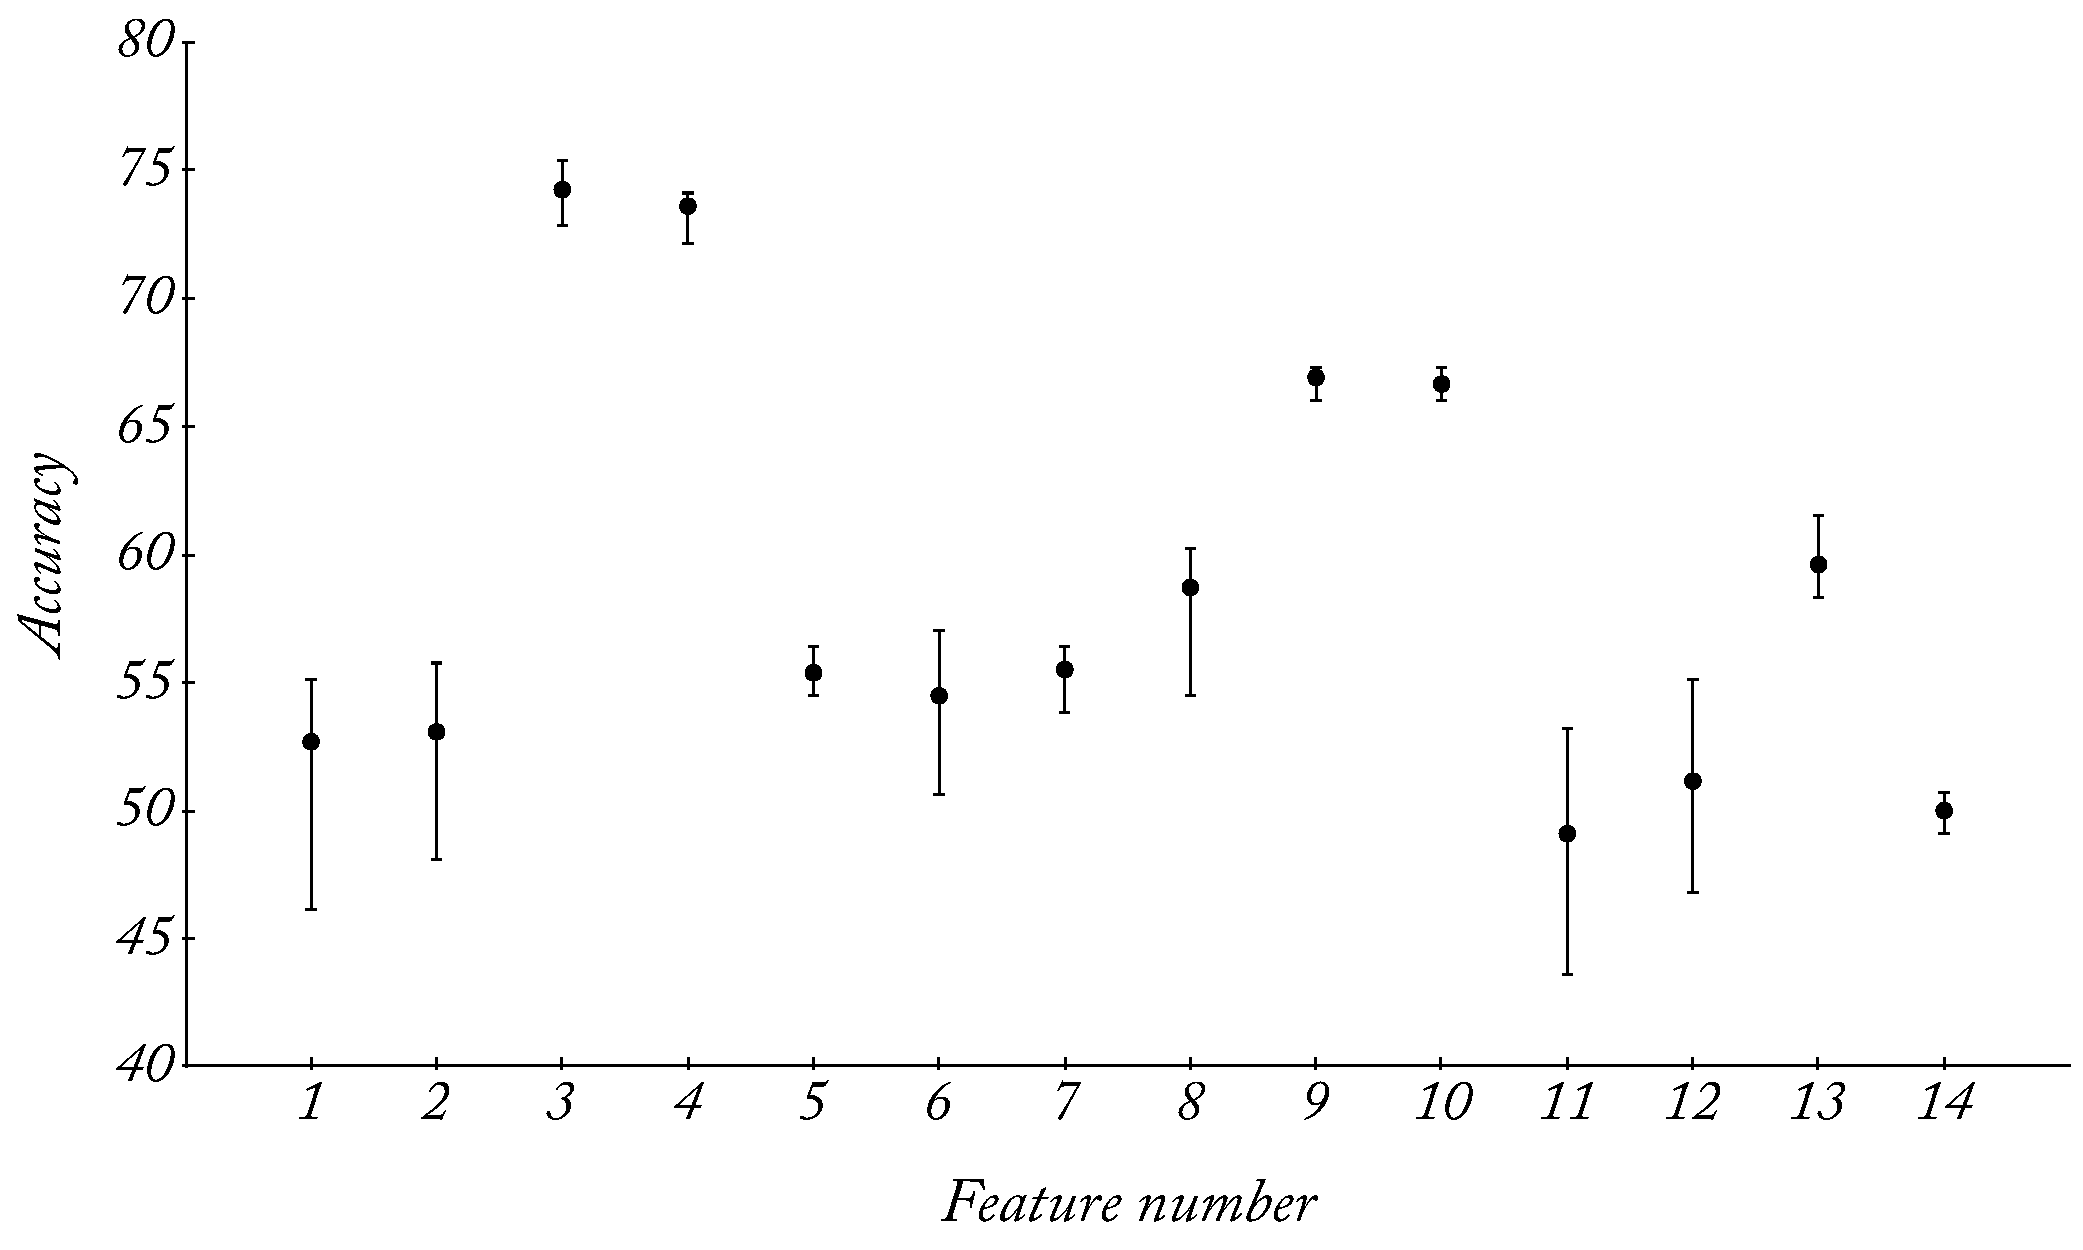
\includegraphics[width=1.0\textwidth]{graphs/subj_a.pdf}
\end{figure}

We found that URLs and strong subjectives clues were the most informative feature in terms of accuracy. URLs are clearly the most discriminative feature, and when used as a presence-based feature heralded an average classification accuracy of 72.84\%. The presence of strong subjective clues also served as a particularly discriminative feature, classifying 66.9\% of examples correctly when used as a presence-based feature. Furthermore, when used as individual features, we found that URLs and strong subjective clues presented little spread in our accuracy results. This suggests that unlike features such as adjectives or weak subjective clues, URLs and strong subjective clues are not sensitive to changes in training data. Interestingly however, we also found that there was little change in accuracy when basing a feature on presence or number of occurrences within the status. All our features, other than weak subjective clue presence, resulted in accuracies greater than 50\%. As such, although some do little better than simply guessing, most offer at least some additional insight when classifying a status' subjectivity.

\begin{figure}
	\caption{Precision average and spread for each individual feature}
	\label{fig:subj_p}
	\centering
		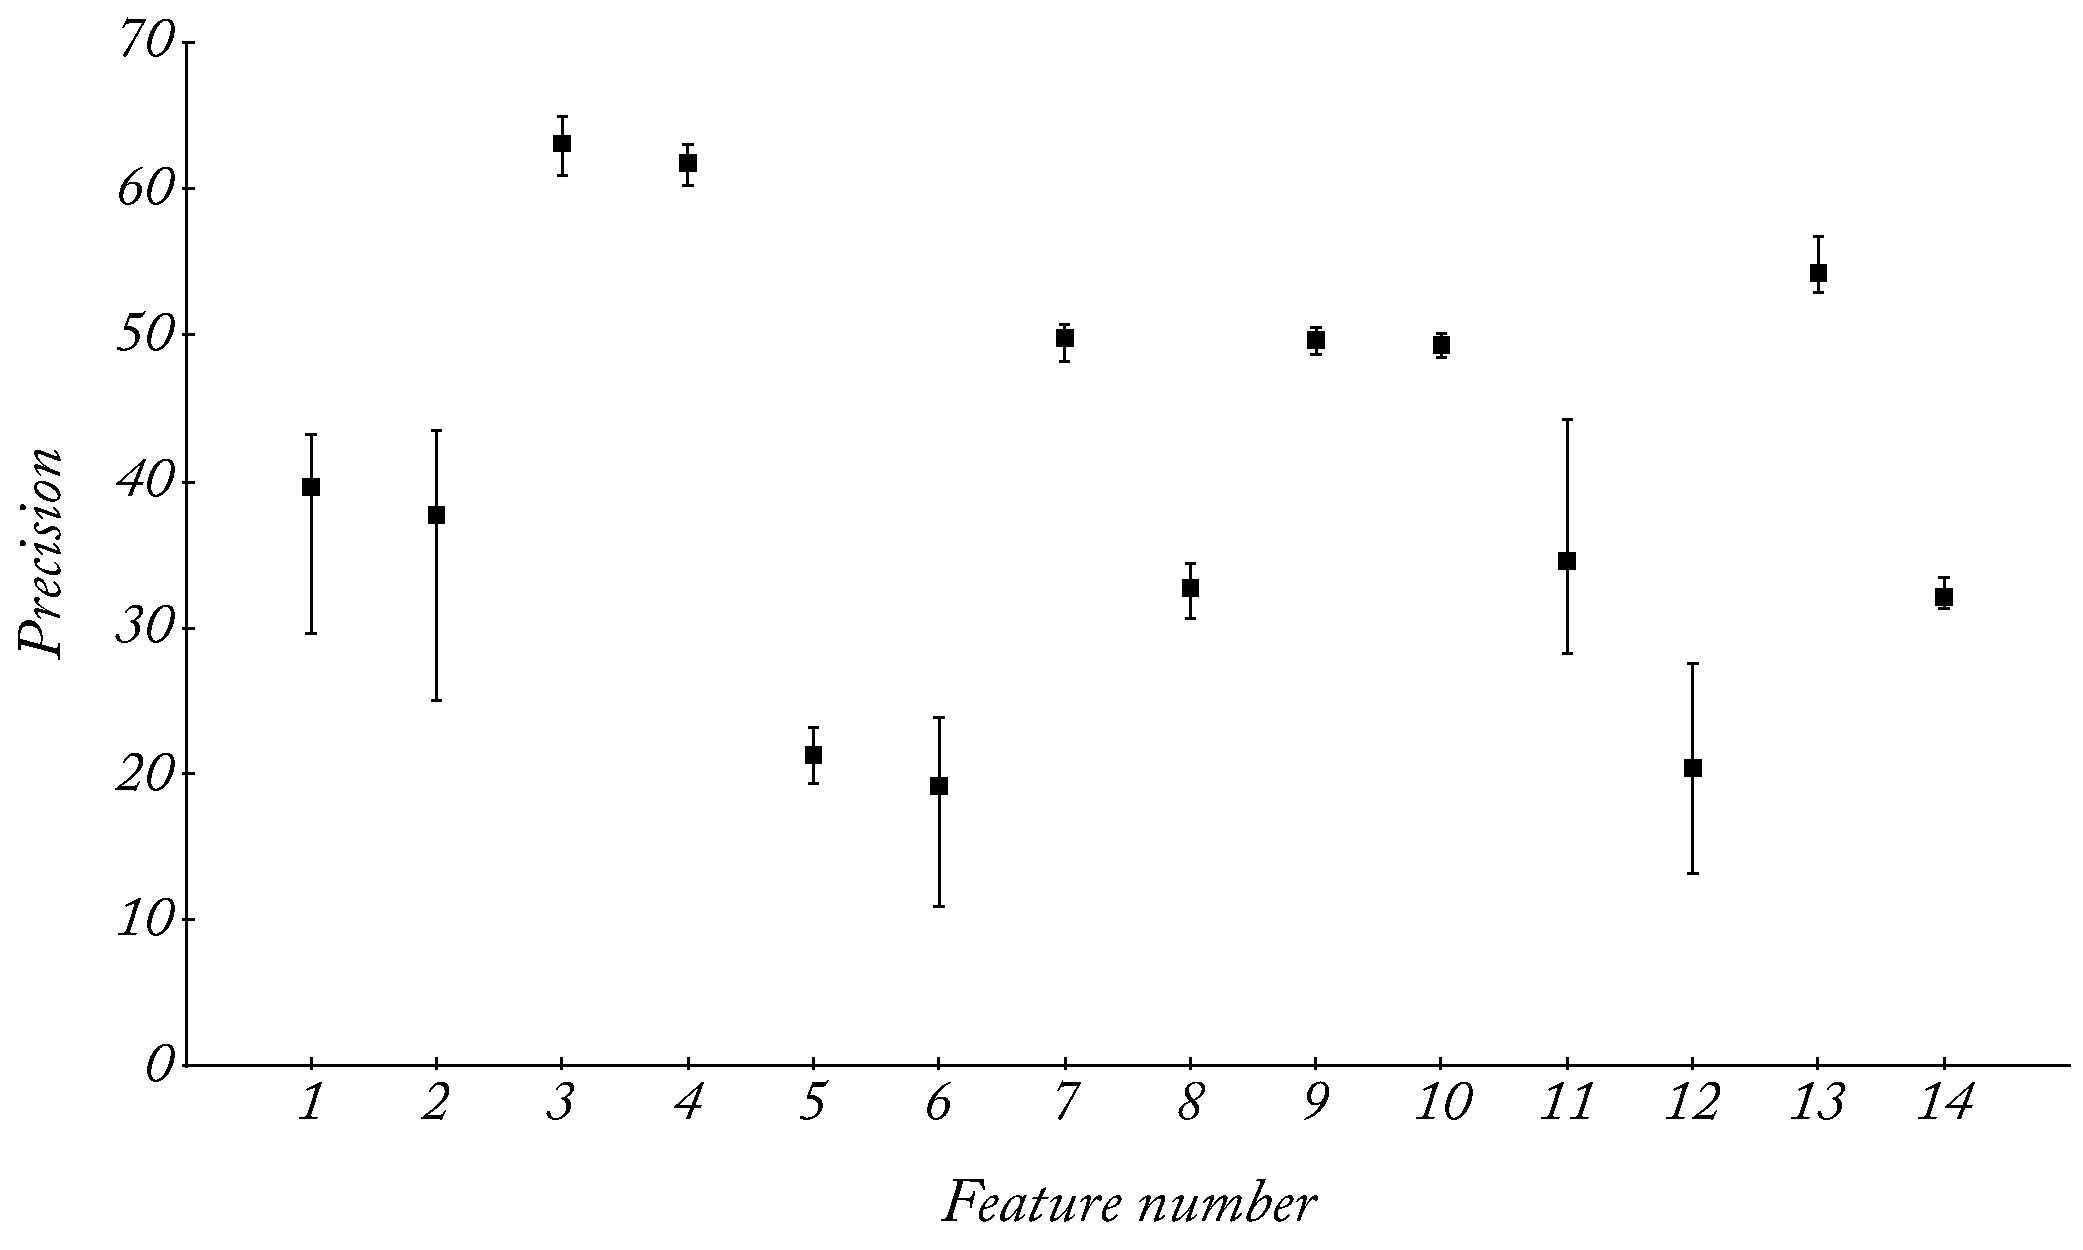
\includegraphics[width=1.0\textwidth]{graphs/subj_p.pdf}
\end{figure}

In general, we found that features on their own presented little in the way of precision. As with accuracy, URLs again offered the best as far as precision rates were concerned, with precision rates of 63.1\% when used as a presence-feature and 61.8\% when the number of occurrences was taken into account. Also of note was our capitalised words feature which achieved a precision rate of 54.3\%. Again weak subjectives performed weakly as a feature, and both it and adjectives suggested that their sensitivity to changes in training data made them unreliable.

\begin{figure}
	\caption{Recall average and spread for each individual feature}
	\label{fig:subj_r}
	\centering
		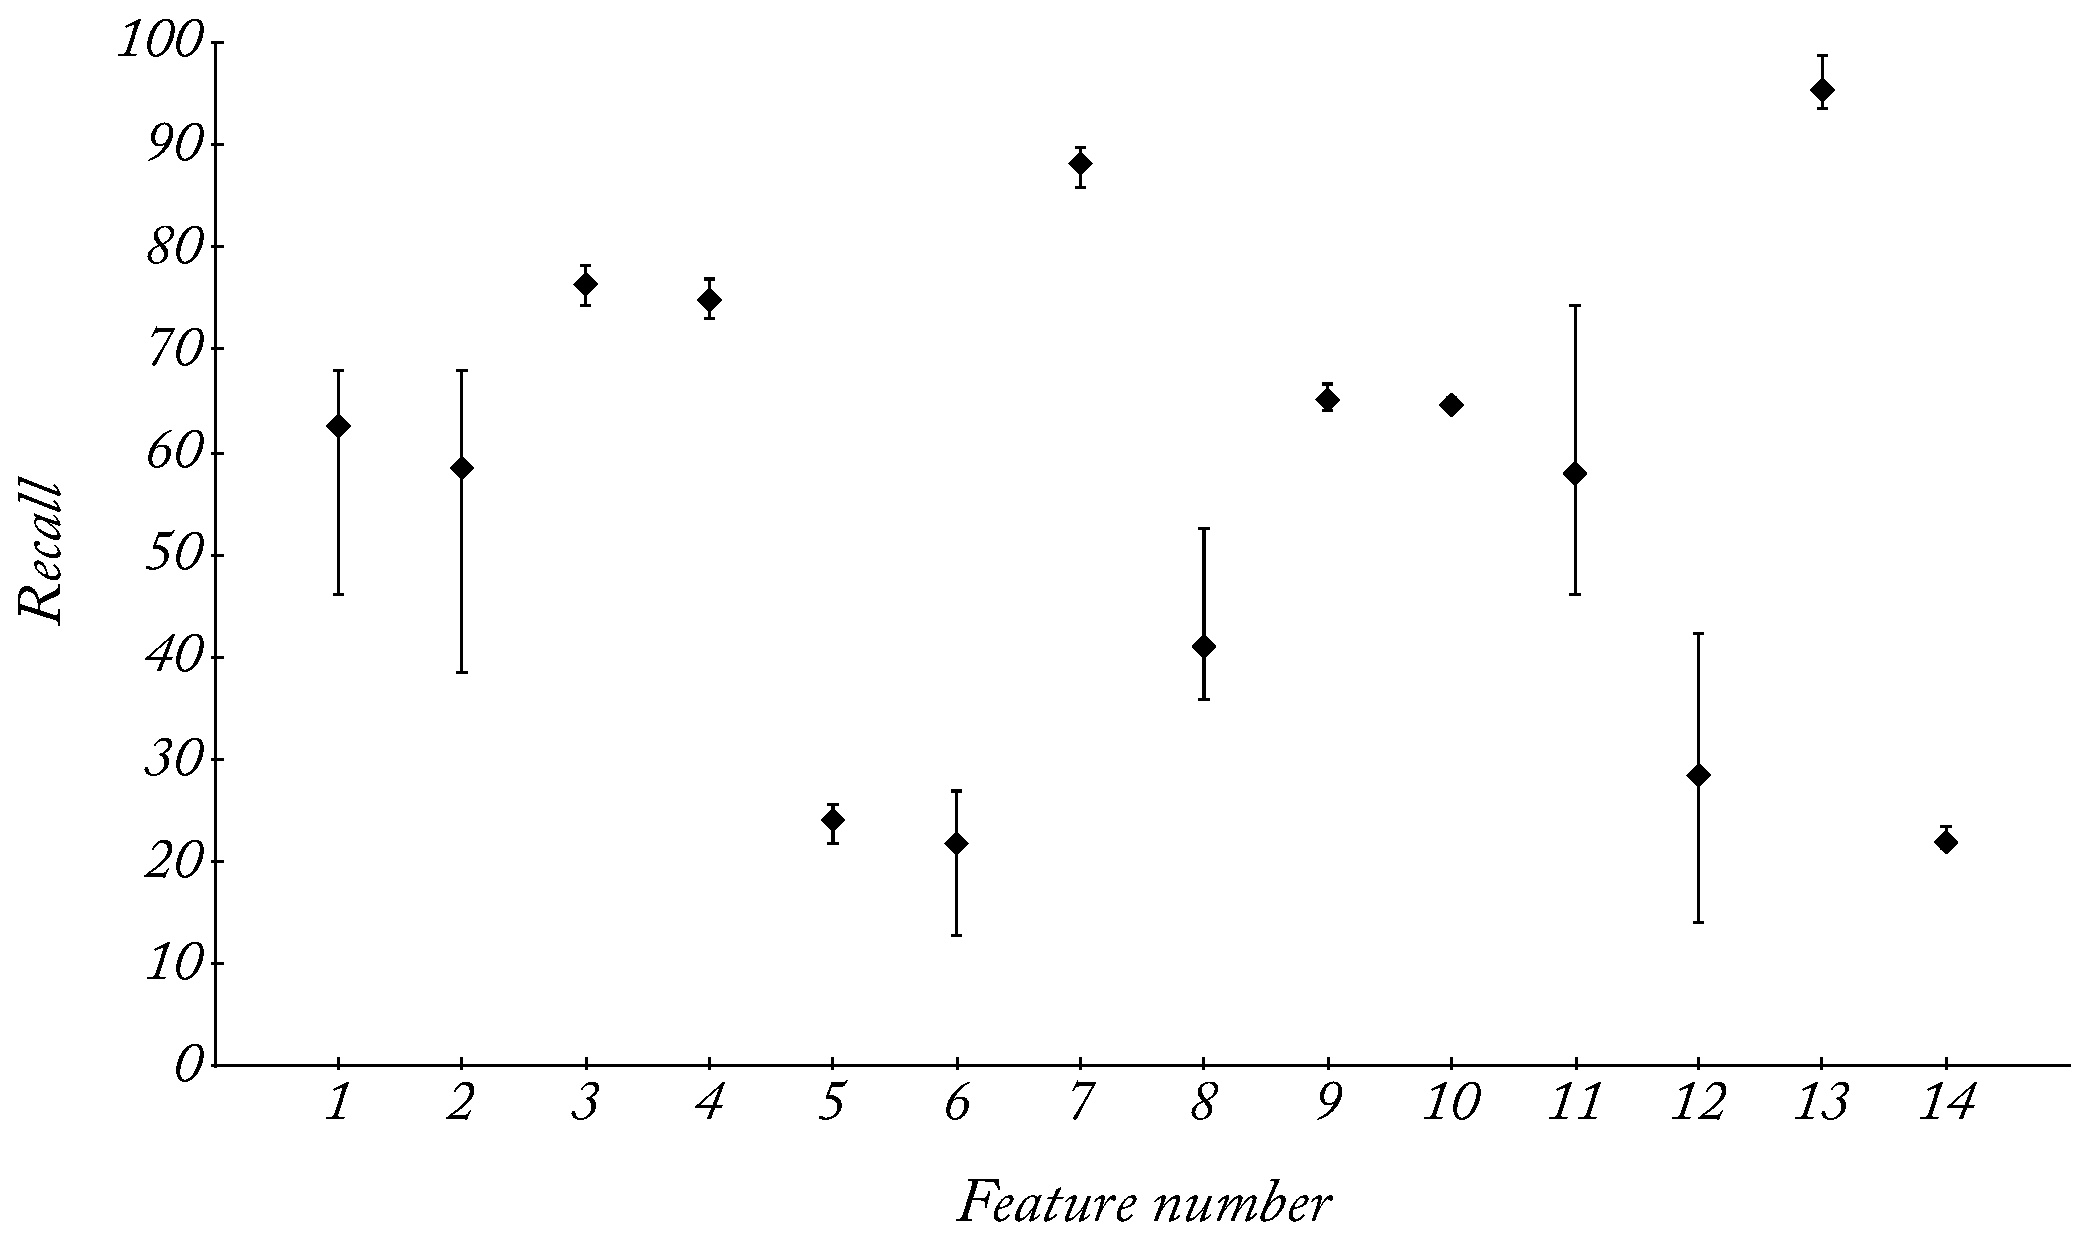
\includegraphics[width=1.0\textwidth]{graphs/subj_r.pdf}
\end{figure}

Recall rates proved much better for our features. This is probably largely due to the one sided-ness of much of their classification, especially in the case of capitalised words, which labelled almost 100\% of its test data as subjective. Of note however are the high recall rates achieved by URLs and strong subjective clues, which we had already identified as strong potential features. Again adjectives and weak subjective clues demonstrated their tendency to be strongly affected by changes in training data, suggesting their potential unsuitability for subjectivity classification. For adjectives, this is strongly at odds with prior research in the field, and as a result we will further experiment with it when testing how our classifier performs with groups of features.

\subsection{Feature set performance}
\label{subjectivity:feature_set}

As a result of our individual feature analysis, we put forward five feature-combinations for further testing:

\begin{enumerate}
	\item has\_urls?, has\_strong\_clues?
	\item has\_urls?, has\_strong\_clues?, no\_clues
	\item has\_urls?, has\_strong\_clues?, capitalised\_words\_frequency
	\item has\_urls?, has\_strong\_clues?, no\_clues, capitalised\_words\_frequency
	\item has\_urls?, has\_strong\_clues?, no\_clues, capitalised\_words\_frequency, has\_adjectives?
\end{enumerate}

The results of our tests using the five feature sets are listed in figure \ref{fig:subj_multi}. Blue bars represent precision, red represents accuracy and green represents recall.

\begin{figure}
	\caption{Precision (square), accuracy (circle) and recall (diamond) results for our five different feature sets.}
	\label{fig:subj_multi}
	\centering
		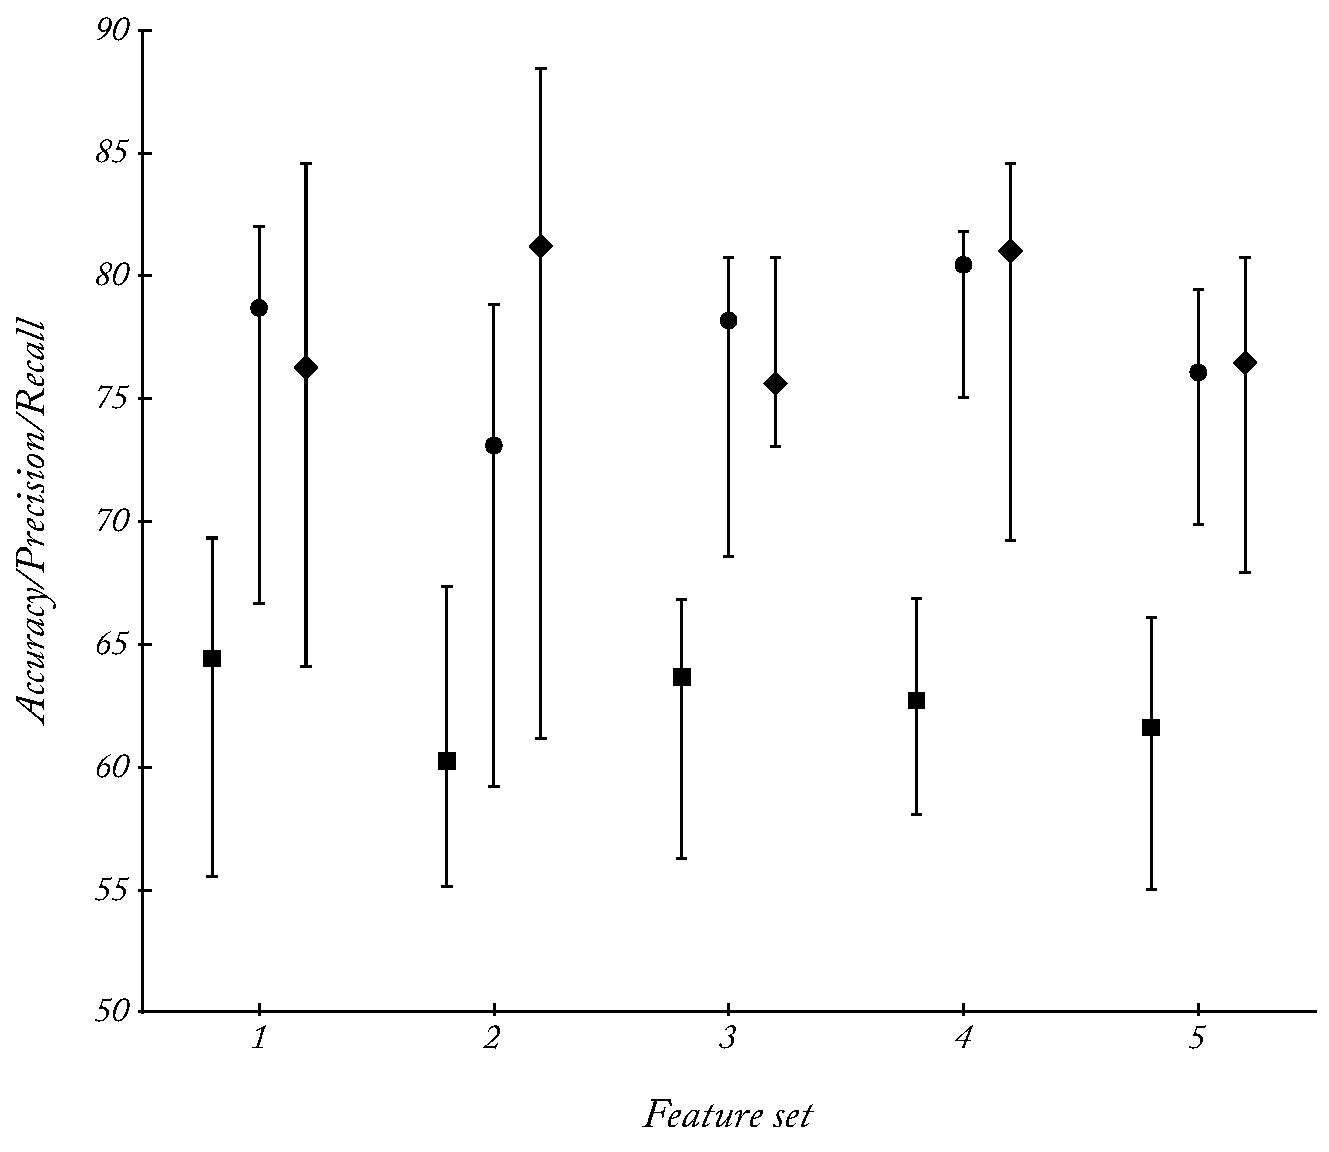
\includegraphics[width=0.9\textwidth]{graphs/subj_multi.pdf}
\end{figure}

All classifiers perform well, with our fourth feature set performing strongest in terms of accuracy achieving an average of 80.5\%. It performed marginally worse that feature set two with regards to precision, scoring an average of 81.0\%. Although it's precision was not the best, its strong accuracy and recall, combined with it's low sensitivity to changes in the training set, make it our preferred feature set. Interestingly adjectives seemed to have an adverse effect on our overall accuracy, precision and recall.

\subsection{Classifier type}

In order to determine the most appropriate classifier type, we ran our tests using a Support Vector Machine for one test and a Naive Bayes Classifier for the other. When building our classifiers, we used the fourth feature set from section \ref{subjectivity:feature_set}. We present our results in figure \ref{fig:subj_class}.

\begin{figure}
	\caption{Precision (square), accuracy (circle) and recall (diamond) results for SVM and NB classifier.}
	\label{fig:subj_class}
	\centering
		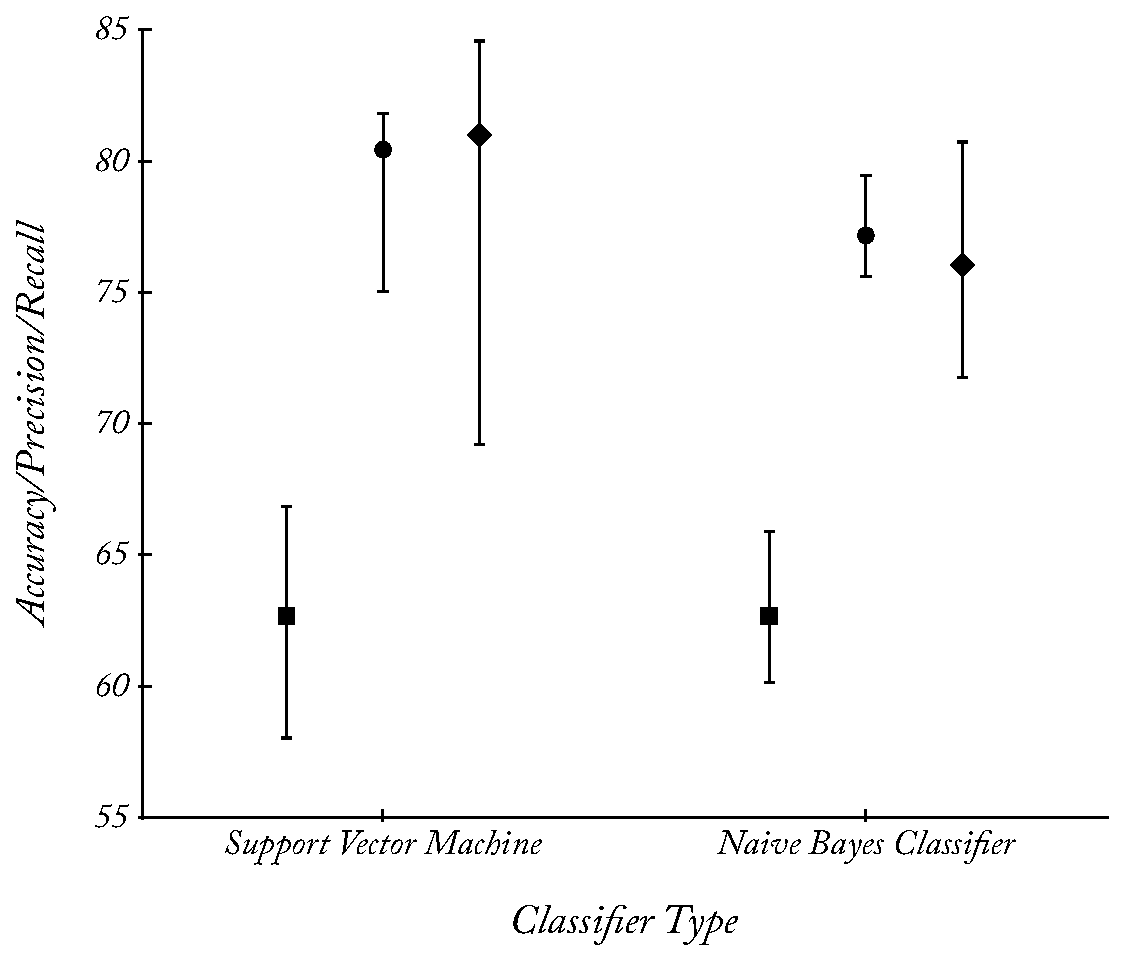
\includegraphics[width=0.8\textwidth]{graphs/subj_class.pdf}
\end{figure}

In terms overall performance, there is little difference between our SVM and NB performance. Overall SVM slightly outperforms NB in terms of accuracy with an average of 72.7\% against the NB average of 71\%. We feel however that in the future if the amount of training data we have is to increase, the SVM would provide a more robust and useful classification method.

\section{Evaluation}

Our subjectivity classification rates were strong. With an average accuracy of 80.5\%, our classifiers performance further improved upon results typically seen in the field, such as the average accuracy of 70.2\% seen by Wiebe et al. \cite{Wiebe:2000tk}. The class itself was both simple to use, and train, though this was largely due to the success of our \emph{Classifier} class implementation. We used a good blend of both linguistic features and Twitter meta-features such as URLs, and as a result saw strong classification rates.

In future work there are five areas in particular which we would look to for further improvement,

\begin{description}
	\item [Training set size] - Overall we felt that the limited size of our training set limited our classifiers ability. In future work we would spend more time building up a much more significant amount of labelled data.
	\item [Word-sense disambiguation] - Although we use part-of-speech tagging to distinguish between the grammatical usage of words, word-sense disambiguation may have seen a further improvement in results. In distinguishing between the senses of words, we provide ourselves with a more dtailed account of their use and are thus better informed when classifying subjectivity.
	\item [No URL feature] - The presence of URLs proved to be a highly discriminative feature when classifying subjectivity. Unlike most other subjectivity classifiers which never come across URLs within their domain, we were able to use this as a feature. We felt that as this was such a dominant feature, its usage both benefitted our classification, but perhaps decreased its linguistic credibility. In future work, we would like to experiment with other features so as not to use URLs which we felt biased our classifier.
	\item [Objective, but opinion] - In examining our objective statuses, we found that there were occasionally objective statuses and links, which although objective, inferred opinion. In future work we hope to examine ways in which a third classification might be introduced for objective statuses which imply opinion.
	\item [Spam classification] - Within our current implementation spam is labelled as objective. As the purpose of our classifier was to help identify opinion, this wasn't a problem, however in future work if we want to make better use of our objective data, a third spam label would be an interesting addition.
\end{description}



	
	\chapter{Sentiment classification}
\label{sentiment}
	
	\chapter{Topic extraction}
\label{topic}

With our statuses' sentiment now classified, we can now look to better understanding the targets and key themes within it. Our approach to topic extraction hopes to identify key words and topics, thus the term topic extraction is used loosely. Our approach hopes to observe and extract the grammatical patterns of keywords within our training data, and use those in turn to extract key words and topics from previously unseen statuses. Although we do not want incorrect keywords, as our ultimate aim is to identify similar statuses through matching topics, to a certain extent we are less worried in identifying too many topics, than we are with identifying too few.

\section{Extracting patterns}

In order to build up a set of topic extraction patterns, we first had to annotate our data in a suitable manner. We added an additional \texttt{topics} attribute to our trained status objects, allowing us to specify an array of topics. Each topic can be one or more words, but must be annotated as it is represented in the data. For example, if we were to annotate \emph{Example 3}, we might select "\emph{Obama}", "\emph{European debt crisis}" and "\emph{US}" as its core topics and keywords. However in labelling the status, we could not for example use "\emph{Europe's debt crisis}" as a topic, as it does not represent how the topic is actually expressed within the status.

Our patterns hope to identify the part of speech structures used to express topics within statuses. In order to do this we look to extract the parts of speech used to express the topic, along with the parts of speech for the two words which precede and follow the topic itself. Thus using the topics we selected for \emph{Example 3}, we might observe the following patterns:

\begin{enumerate}
	\item \emph{Obama}: \texttt{[nil, "nnp", "vbz"]}
	\item \emph{European debt crisis}: \texttt{["vbz", "jj", "nn", "nn", "md"]}
	\item \emph{US}: \texttt{["nn", "nnp", "rb"]}
\end{enumerate}

In order to achieve this, we must first identify each annotated topic within our parts of speech array. This is done by first noting the word length, $n$ of the topic being identified, before then splitting the parts of speech into its n-grams. With a series of n-length phrases now available, it is simply a matter of iterating through each n-gram and checking whether it matches our topic phrase. If so the parts of speech are noted, and the pattern returned. We wrap this up within the \emph{TopicExtraction}'s \texttt{extract\-\_pattern\-(topic,pos)} method, as shown in listing \ref{topic:pattern_extract}.

Thus, for every labelled status, we extract its annotated topic's part of speech pattern, building an overall set of rules which help identify topics within previously unseen statuses. We store theses patterns in our \emph{TopicExtraction}'s class level array, \texttt{patterns}.

\section{Identifying patterns}

With our patterns now identified, we need to define a method to identify them within any given status. This is done by making use the Ruby \emph{Array} object method, \texttt{include?\-(object)}, which returns a boolean value indicating whether an object occurs within an array. Using the maximum pattern length, we create a collection of n-grams for our status using values of n ranging from three to the said length. For each n-gram we then proceed to check whether it's part of speech tags match any pattern within our \texttt{patterns} array, using the aforementioned \texttt{include?\-(object)} method. If the n-gram does exist, its first and last elements are removed, and the remaining topic is returned. This method is wrapped up in the class level \texttt{extract\-\_topics\-(status)} method, which returns an array of topics. We have included the method code in listing \ref{topic:topic_extract}.

\section{Evaluation}

Our topic extraction module proved an effective way of gathering keywords and topics for statuses. Although difficult to assess quantitatively, we found that in manually examining the results our extraction engine almost always identified the core topics. In some cases it was slightly overzealous in identifying topics, and future work might look at how we can ensure it identifies a slightly more concise set of topics. Nonetheless the results were accurate, and in general did not omit any important topics when attempting to extract them. 

As research into topic extraction tends to be carried out for a whole gamut of purposes, it is difficult to asses our performance in comparison to others. Overall however, we felt that our topic extraction module performed well and perfectly suited the needs of our project.
	
	\chapter{Software engineering}

Lorem ipsum dolor sit amet, consectetur adipisicing elit, sed do eiusmod tempor incididunt ut labore et dolore magna aliqua. Ut enim ad minim veniam, quis nostrud exercitation ullamco laboris nisi ut aliquip ex ea commodo consequat. Duis aute irure dolor in reprehenderit in voluptate velit esse cillum dolore eu fugiat nulla pariatur. Excepteur sint occaecat cupidatat non proident, sunt in culpa qui officia deserunt mollit anim id est laborum.
	
	\chapter{Testing}

Lorem ipsum dolor sit amet, consectetur adipisicing elit, sed do eiusmod tempor incididunt ut labore et dolore magna aliqua. Ut enim ad minim veniam, quis nostrud exercitation ullamco laboris nisi ut aliquip ex ea commodo consequat. Duis aute irure dolor in reprehenderit in voluptate velit esse cillum dolore eu fugiat nulla pariatur. Excepteur sint occaecat cupidatat non proident, sunt in culpa qui officia deserunt mollit anim id est laborum.
	
	\part{Evalutation}
	
	% Be warned that many projects fall down through poor evaluation. Simply building a system and documenting its design and functionality is not enough to gain top marks. It is extremely important that you evaluate what you have done both in absolute terms and in comparison with existing techniques, software, hardware etc. This might involve quantitative evaluation, for example based on numerical results, performance etc. or something more qualitative such as expressibility, functionality, ease-of-use etc. At some point you should also evaluate the strengths and weaknesses of what you have done. Avoid statements like "The project has been a complete success and we have solved all the problems asssociated with blah...; - you will be shot down immediately! It is important to understand that there is no such thing as a perfect project. Even the very best pieces of work have their limitations and you are expected to provide a proper critical appraisal of what you have done.

\chapter{Evaluation}

As each component has been evaluated in its respective chapter, within this chapter we shall instead evaluate to what extent our original project aims have been met. We shall first examine those discussed within our core aims, before finally evaluating to what extent our secondary aims were met.

\section{Core aims}

\subsection{Sentiment analysis engine}

\begin{enumerate}
		\item \emph{A Twitter scraper which will fetch live statuses from Twitter.} \\
		Our content retrieval module draws live data from the size in an effective and stable manner. Statuses are pre-processed and stored in MongoDB, whilst our Status class provides a simple interface for accessing the data from within Ruby.
		\item \emph{A method for determining whether fetched statuses are opinionated or not.} \\
		Our subjectivity classifier performs strongly in identifying opinionated text, and serves as an effective tool for doing this. We feel that our blend of existing research with Twitter focussed aspects worked well, and our accuracy rates are better than those seen in literature.
		\item \emph{A method for identifying whether fetched statuses' opinion is positive or negative.} \\
		Our polarity classifier serves as an effective tool for determining polarity. Its classification accuracy is on par with others in literature, although there are some which marginally outperform ours. We feel that this is largely due to our limited training set size, and future work would place a much larger focus on building this.
		\item \emph{A method for identifying the core topics which our fetched statuses are discussing.} \\
		Our topic extraction module performs well within the context of our project, and serves as a useful tool for drawing together statuses whose focus is similar.
		\item \emph{A means of persisting our statuses and the results of the above methods, such that they can be easily retrieved at any time.} \\
		As discussed in our first point, the MongoDB store serves as a robust store for our data and the Status class makes accessing its data simple. 
\end{enumerate}

\subsection{Web services}

\begin{enumerate}
	\item \emph{Requests can be made to classify a status, upon which the service should return the classification engine's results.} \\
	Our classification web service provided a simple to use way for external developer to make use of our sentiment analysis engine. Response times were fast, and the formatted JSON results made computer interpretation simple.
	\item \emph{A method for requesting any classified data our engine may have stored.} \\
	Our results web service provided an easy way of accessing our live, and past, results. The parameters allowed developers to tailor the results they were retrieving, so that only information relevant to them was returned. Furthermore, as with our classification web service, response times were fast and the JSON results made computer interpretation simple.
\end{enumerate}
	
\section{Additional aims}

\begin{enumerate}
	\item \emph{Extend our sentiment analysis engine to give a more detailed account of a broader spectrum of emotion.} \\
	Little research has been conducted into emotion classification. We felt that our emotion classifier presented an innovative and unique take on emotion classification. The assigned emotion labels were in general close to our own manual annotations, and we felt that it provided a viable and effective method for classification.
	\item \emph{Web based visualisation tool for better understanding and exploring sentiment on Twitter.}
	Our visualisation tool was an innovative and uniqe way of exploring opinion. It presented our detailed results in a simple and fluid manner, along with making the results easily accessible to all.
\end{enumerate}

\section{Summary}

In summary we feel that the project met all of its goals with in general a great deal of success. Our subjectivity classifier performed well, and although our polarity classifier was not perfect, we feel that the we have identified the changes required to improve it. Our exploration into emotion classification proved insightful, and the results were promising. Our topic extraction engine serves its purpose within the project and managed to identify core topics well. Additionally, we felt that the engine has a whole was fairly extensible, and our approach to its design means that using it with other micro-blogging services should be simple. Finally, we felt that our overall delivery methods were simple to use, and managed to mask the complexity of the tasks they were interfacing to well.
	
	\chapter{Conclusion}
\label{conclusion}
% The project's conclusions should list the things which have been learnt as a result of the work you have done. For example, "The use of overloading in C++ provides a very elegant mechanism for transparent parallelisation of sequential programs", or "The overheads of linear-time n-body algorithms makes them computationally less efficient than O(n log n) algorithms for systems with less than 100000 particles". Avoid tedious personal reflections like "I learned a lot about C++ programming...", or "Simulating colliding galaxies can be real fun...". It is common to finish the report by listing ways in which the project can be taken further. This might, for example, be a plan for doing the project better if you had a chance to do it again, turning the project deliverables into a more polished end product, or extending the project into a programme for an MPhil or PhD.
	
	% BIBLIOGRAPHY
	% This consists of a list of all the books, articles, manuals etc. used in the project and referred to in the report. You should provide enough information to allow the reader to find the source. In particular references must contain all the information regarding the publication of the paper and must be consistently formatted. Usually this means:
	% For journals: Authors, Title, Journal, volume number, issue number, page number, publisher, month, year.
	% For conferences: Authors, Title, Conference name, Place where held, publisher, page number, month, year.
	% For technical reports: Authors, Title, institution, Technical report number, month, year.
	% For web references: Authors, Title, Web-reference, date accessed.
	% URLs are optional for published work but preferred.
	% A weakness of many reports is inadequate citation of a source of information. It's easy to get this right so there are no excuses. Each entry in the bibliography should list the author(s) and title of the piece of work and should give full details of where it can be found. For example:
	% 1 Bennett, A.J., Field, A.J. and Harrison, P.G., "Modelling and Validation of Shared Memory Coherency Protocols", Performance Evaluation, 1996, Vol. 27 & 28, 1996, pp. 541-562.
	

	\bibliographystyle{plain}
	\bibliography{papers,web}	

\end{document}


